%
% This LaTeX source file provides a template for a typical research paper.
%

%
% Use the standard article template.
%
\documentclass{article}
% Copyright 2017 Sergei Tikhomirov, MIT License
% https://github.com/s-tikhomirov/solidity-latex-highlighting/

\usepackage{listings, xcolor}

\definecolor{verylightgray}{rgb}{.97,.97,.97}

\lstdefinelanguage{Solidity}{
	keywords=[1]{anonymous, assembly, assert, balance, break, call, callcode, case, catch, class, constant, continue, contract, debugger, default, delegatecall, delete, do, else, emit, event, export, external, false, finally, for, function, gas, if, implements, import, in, indexed, instanceof, interface, internal, is, length, library, log0, log1, log2, log3, log4, memory, modifier, new, payable, pragma, private, protected, public, pure, push, require, return, returns, revert, selfdestruct, send, storage, struct, suicide, super, switch, then, this, throw, transfer, true, try, typeof, using, value, view, while, with, addmod, ecrecover, keccak256, mulmod, ripemd160, sha256, sha3}, % generic keywords including crypto operations
	keywordstyle=[1]\color{blue}\bfseries,
	keywords=[2]{address, bool, byte, bytes, bytes1, bytes2, bytes3, bytes4, bytes5, bytes6, bytes7, bytes8, bytes9, bytes10, bytes11, bytes12, bytes13, bytes14, bytes15, bytes16, bytes17, bytes18, bytes19, bytes20, bytes21, bytes22, bytes23, bytes24, bytes25, bytes26, bytes27, bytes28, bytes29, bytes30, bytes31, bytes32, enum, int, int8, int16, int24, int32, int40, int48, int56, int64, int72, int80, int88, int96, int104, int112, int120, int128, int136, int144, int152, int160, int168, int176, int184, int192, int200, int208, int216, int224, int232, int240, int248, int256, mapping, string, uint, uint8, uint16, uint24, uint32, uint40, uint48, uint56, uint64, uint72, uint80, uint88, uint96, uint104, uint112, uint120, uint128, uint136, uint144, uint152, uint160, uint168, uint176, uint184, uint192, uint200, uint208, uint216, uint224, uint232, uint240, uint248, uint256, var, void, ether, finney, szabo, wei, days, hours, minutes, seconds, weeks, years},	% types; money and time units
	keywordstyle=[2]\color{teal}\bfseries,
	keywords=[3]{block, blockhash, coinbase, difficulty, gaslimit, number, timestamp, msg, data, gas, sender, sig, value, now, tx, gasprice, origin},	% environment variables
	keywordstyle=[3]\color{violet}\bfseries,
	identifierstyle=\color{black},
	sensitive=false,
	comment=[l]{//},
	morecomment=[s]{/*}{*/},
	commentstyle=\color{gray}\ttfamily,
	stringstyle=\color{red}\ttfamily,
	morestring=[b]',
	morestring=[b]"
}

\lstset{
	language=Solidity,
	backgroundcolor=\color{verylightgray},
	extendedchars=true,
	basicstyle=\footnotesize\ttfamily,
	showstringspaces=false,
	showspaces=false,
	numbers=left,
	numberstyle=\footnotesize,
	numbersep=9pt,
	tabsize=2,
	breaklines=true,
	showtabs=false,
	captionpos=b
}


% The geometry package allows for easy page formatting.
\usepackage{geometry}
\geometry{letterpaper}

% Load up special logo commands.
\usepackage{doc}

% Package for formatting URLs.
\usepackage{url}

% Packages and definitions for graphics files.
\usepackage{graphicx}
\usepackage{epstopdf}

\usepackage{subcaption}
\usepackage{booktabs}

\DeclareGraphicsRule{.tif}{png}{.png}{`convert #1 `dirname #1`/`basename #1 .tif`.png}

%
% Set the title, author, and date.
%
\title{Blockchain in Smart Mobility \\ \large Decentralized Car Marketplace}
\author{Lucas Rebscher, Robin Papke, Hai Duc Dang, Chinh Tran}
\date{}

%
% The document proper.
%
\begin{document}

% Add the title section.
\maketitle

% Add an abstract.
\begin{abstract}
Besides being the foundation of most popular cryptocurrencies, blockchain also promises to be a disruptive technological concept for various areas such as smart mobility. Blockchain enables new use cases and business possibilities that might benefit from the advantages that the technology provides.
In this work, we present an implementation of a decentralized car marketplace based on the Ethereum platform. By leveraging the idea of digital assets and the temper-proof nature of blockchains, we can provide assurances regarding vehicle information to customers. The results show that our smart contracts can cover core features of a car marketplace. Additionally, they enable customer trust and allow a secure ownership transfer without an intermediary third-party. However, there are still challenges that have to be addressed in future work.
\end{abstract}


% Add various lists on new pages.
\pagebreak
\tableofcontents

\pagebreak
\listoffigures

\pagebreak
\listoftables

% Start the paper on a new page.
\pagebreak

\section{Introduction}
In the course of this work we evaluate an example implementation of a car marketplace based on blockchain technology. We start this introduction with context on how blockchain has become such a popular topic in recent years. Afterwards, we will discuss the purpose of this work as well as our objectives. We will also introduce some other similar applications that already made efforts to leverage the advantages of blockchains.

\subsection{Motivation}
The progressive technological development of the last decades has led to the emergence of massive amounts of data that were hardly imaginable in the past. More and more information is being digitized daily, including personal data. The secure management of this data, especially private data, is a challenging task and has been a source of concern for some time. Most people cannot conclusively determine how their data is handled once it has been handed over, leading to insecurity and discontent. Regardless of which management solution a third party actually uses to handle user data, users will always need a certain degree of trust before entrusting their sensitive data to someone else. One example in which trust in data is particularly important are car marketplaces. Customers need to be certain that vehicle information provided by a platform has not been altered to mislead them into buying an improperly advertised vehicle.

In 2008 Satoshi Nakamoto \cite{nakamoto2008bitcoin} first presented Bitcoin, an approach for a peer-to-peer electronic cash system using a public transaction ledger, also called blockchain. With this ledger, he is able to provide secure transactions between two parties without requiring any trust. This idea directly addresses the data privacy concerns that many people currently share. As a result, blockchain technology has sparked great interest as it could potentially improve the current state of data privacy in our society. Other popular blockchain technologies such as Ethereum \cite{Ethereum} are already working on advancing this idea and enable developers to leverage blockchains in both new as well as existing applications.

For this reason, it is of great interest to dive deeper into the theoretical concepts behind blockchains to see how they address the above-mentioned issues. At the same time, it is important to put this idea into a practical context, such as a car marketplace, and evaluate its potential impact.

\subsection{Problem Statement}
Despite the great interest and potential of blockchains, this rather new technology has not yet been widely adopted. On the one hand, people new to this type of technology may not have the time or the desire to work through the multitude of available resources to attain a level of confidence to use blockchain-based services themselves. This issue may be amplified by the large amount of information revolving around new blockchain-based technologies that is circulating the media on a daily basis. On the other hand, companies may not have yet the incentive, that would justify spending time and resources to deploy blockchains internally or in their products.

\subsection{Contribution}
In the course of this work we evaluate the application of blockchains for software development presenting a sample implementation of a blockchain-based car marketplace. In our application we utilize the open-source blockchain platform Ethereum \cite{Ethereum}. By using smart contracts, we can manage data in a secure manner. Adding this component to our otherwise more traditional architecture we are able to leverage the advantages of blockchains while building upon already existing ideas.

This work provides both a theoretical introduction to the topic of blockchains as well as insights to the implementation of applications based on blockchain. This may assist readers to further pursuit the subject of blockchains both theoritically and practically. Additionally we discuss the potential advantages of our application over more traditional approaches. As a result of this work, readers may be able to better reflect on their own ideas.

\subsection{Related Work}
Many people have already made great efforts to use blockchains and to extend or implement new applications based on them. One of these applications is LBRY \cite{lbry}, a digital marketplace that is not controlled by a central authority but by its participants instead. Users providing content on this platform are directly associated with that content and have control over it. LBRY uses blockchain technology to store and lookup decentralized metadata. An user can store his data in this blockchain by bidding on LBRY names. The owner of such a name is in control over its content as well as its access rights. Another platform that involves cars and uses blockchain technology is carVertical \cite{carVertical} which allegedly enables users to perform a decentralized vehicle check using blockchain. Among other things, this may be used to browse the history of a vehicle or to check whether a vehicle has been stolen. BitCar \cite{BitCar} is another blockchain-based platform that involves car assets. On this platform, users can allegedly trade fractional ownerships of cars and possibly aquire complete ownership of luxury cars.

\subsection{Outline}
The rest of this paper is divided into seven sections. In Section~\ref{sec:foundations} we present the theoretical foundations to blockchains, which will help the reader to understand the core concepts of the topic. In Section~\ref{sec:concept} we discuss the general concepts of our example implementation and describe the requirements and assumptions. Based on these concepts, we describe our implementation and explore the technical aspects  in Section~\ref{sec:impl}. This includes the smart contracts, data structures and data flow in our application. The selling points of our prototype are discussed in Section~\ref{sec:selling_points}.
Finally, Section~\ref{sec:conclusion} summarizes our work, mentions some of the remaining challanges and provides a future perspective on the topic.

\clearpage
\section{Foundations} \label{sec:foundations}

\subsection{Blockchain}
The term blockchain still has no satisfying definition yet, but the ISO/TC 307 describes a blockchain as the following:
[Blockchain is] \textit{a shared, immutable ledger that can record transactions across different industries, [...]  It is a digital platform, that records and verifies transactions in a transparent and secure way, removing the need for middlemen and increasing trust through its highly transparent nature}.
\\
\\
In practice, this means that a blockchain is a distributed computer architecture where each computer is treated as a node of this network. Each node has knowledge of all transactions inside the network. Transactions are encrypted and bundled in a so called 'block'. Only one block at a time can be added to the network, because it has to be verified that it follows the previous blocks first. Nowadays, blockchain technologies have the following traits:
\begin{itemize}
\item \textbf{Distributed}: Each node is considered equal and has the full history of all transactions.
Because this ledger isn't stored in a central location, blockchains avoid situations like 'single point of failure', which can be inherent in client-server based system.
\item \textbf{Time-Stamped}: Each block contains a timestamp, along with a cryptographic hash of the previous block and transaction data. Consequently, with each new block it becomes harder to change past entries, because they are built on the information of past blocks.
\item \textbf{Consensus}: Once the block is recorded, a consensus algorithm ensures that the data in any given block cannot retroactively be altered without changing the data of all subsequent blocks. To achieve this, it would require at least 51 percent control of the whole network. This guarantees that a value can only be spent once~\cite{Blockchain}.
\end{itemize}


Due to these traits, blockchain technology makes a suitable fit for storing  medical records, identity management and financial transaction processing~\cite{Application}.

There are two types of blockchains: private and public. The best known public blockchain is the Bitcoin Network, in which everyone is allowed to read and write data to the ledger.
An advantage of such a blockchain type is, that no access control is needed and therefore applications can be built on top of it without the approval of others.
A private blockchain needs a participant to have the appropriate permission, in order to join the network. In contrast to the public blockchains, they do not rely on anonymous nodes to validate transactions, as the validators are vetted by the network owner~\cite{Private}.

\subsection{Consensus Algorithm}

Consensus is a group decision-making process in which group members develop and agree to support a decision in the best interest of the whole. The goal is to ensure the existence of a single source of truth. An overview of well-known consensus algorithms is outlined in Table~\ref{table:consensus}. In the following, we will describe the two most popular consensus algorithms, namely Proof-of-Work and Proof-of-Stake more in detail.

\subsubsection{Proof-of-Work}

Proof-of-Work (PoW) is based on the assumption that work must be put into something to give it value, and in Bitcoin's case this work is doing computations with mining which serves the following two purposes:
\begin{enumerate}
  \item verify the legitimacy of a transaction, or avoiding the so-called double-spending
  \item create new digital currencies by rewarding miners for performing the previous task~\cite{consensus}.
\end{enumerate}

The following steps happen after issuing a transaction:
\begin{itemize}
  \item Transactions are bundled together into what is called a block
  \item Miners verify that transactions within each block are legitimate
  \item Miners solve a mathematical puzzle known as Proof-of-Work problem
  \item A reward is given to the first miner who solves each block's problem
  \item Verified transactions are stored in the public blockchain
\end{itemize}
All the network miners compete to be the first to find a solution for the mathematical problem that concerns the candidate block, a problem that cannot be solved in other ways than through brute force so that essentially requires a huge number of attempts.
When a miner finally finds the right solution, he/she announces it to the whole network at the same time, receiving cryptographic tokens (the reward) provided by the protocol.
From a technical point of view, the mining process is an operation of inverse hashing, i.e. it determines a number (nonce), so the cryptographic hash algorithm of block data results in less than a given threshold~\cite{PoW}.

\subsubsection{Proof-of-Stake}

In contrast to PoW, Proof-of-Stake (PoS) does not use computing power in order to validate transactions, but rather the ownership of the participant's token.
The more tokens an user owns, the higher is the probability to be selected as the new forger.
PoS requires the forger to put his tokens on 'stake' during the validating process, so validating a fraudulent transaction would mean to loose his stake.
Forgers therefore are incentivized to behave according the rules. However, PoS has to deal with the 'Nothing-at-Stake' attack. This problem comes up, if a validator bets on all different proposed versions, thus being certain to win~\cite{PoS}.

\begin{table}[]
\centering
\def\arraystretch{1.5}
\begin{tabular}{@{}p{30mm}p{30mm}p{30mm}p{40mm}p{15mm}@{}}
\toprule
Consensus algorithm              & Resource being used                                                     & Benefits                                                          & Drawbacks                                                                                                                 & Examples          \\ \midrule
Proof-of-Work (PoW)              & Computing power                                                         & Trustless, immutable, highly decentralized                        & High energy consumption, low transaction throughput                                                                       & Bitcoin, Ethereum \\
Proof-of-Stake (PoS)             & Ownership of fixed amount of tokens                                     & Efficient in energy and throughput, scalable                      & Nothing-at-Stake problem, i.e. voting for different forks at the same time                                                & NXT               \\
Delegated PoS                    & Ownership of scarce tokens + peer reputation (election for delegates)   & Allegedly more efficient than PoS                                 & Voter apathy in elections can lead to excessive centralization and reduces robustness                                     & BitShares         \\
Tendermint (Proof-of-Validation) & Security deposit of scarce tokens subject to burn if voting dishonestly & Gives benefits of PoS without almost any of its drawbacks         & Nothing-at-Stake problem still persists over long periods of time                                                         & Eris-DB           \\
Proof-of-Authority (PoA)         & Selected authorities are randomly selected to validate transactions     & Efficient, does not require any inherent tokens or economic value & The corruption of authorities is a large possibility, relies on authorities being well-selected and controlling eachother &                   \\ \bottomrule
\end{tabular}
\caption{Consensus algorithms for usage in blockchains. Adapted from source:
\cite{consensus} with addition of Proof-of-Authority \label{table:consensus}}
\end{table}

\clearpage

\subsection{Ethereum}

Ethereum was the first blockchain technology to incorporate smart contracts~\cite{Ethereum}. These contracts are executed automatically once certain criteria are fulfilled.
Ethereum's initial goal was to ease the creation of decentralized applications. Developers can leverage the Turing-complete programming language to program the arbitrary application logic.
According to the white paper, the main focus was on five key elements:
\begin{itemize}
  \item \textbf{Simplicity}: This characteristic is followed even in some cases for the price of lower storage and time efficiency. No extra complexity is to be brought, only if for fundamental optimization purposes.
  \item \textbf{Universality}: There are no limiting functionalities with Ethereum. Using the internal Turing-complete scripting language which it provides, any use case can be implemented.
  \item \textbf{Modularity}: The Ethereum protocol can be broken up into components which function independently from each other.
  \item \textbf{Agility}: Characteristics of the protocol may be prone to change, however only in cases when it proves to have a high potential for scalability or security.
  \item \textbf{Non-discrimination and Non-censorship}: The implementation of any use case is permitted, a fee is paid for each application running on top of Ethereum.
\end{itemize}
Each transaction contains 'standard' fields that are stored on the ledger, those are: information on the recipient, the signature of the sender, a data field that may be used when deemed so and the number of Ether to be transferred with the transaction.
Apart from these fields, there are two more values: STARTGAS and GASPRICE. These describe the value that are used for computations. Each computation of a transaction costs a certain amount of gas and there is also starting value. This is needed so that no Denial-of-Service (DoS) or other malicious operations leveraging infinite loops can be carried out in the network.

The Ethereum Virtual Machine (EVM) is the environment where the smart contracts are processed during runtime. Therefore, the contract code is compiled into a binary format and then stored in the Ethereum blockchain. The EVM is Turing-complete, meaning that any mathematical computation can be processed by it~\cite{Ethereum}.

\subsubsection{Smart Contracts}
The term smart contract has first been described in an scientific essay of Nick Szabo in 1998, in which he explains how contractual relations between different parties can be secured through computer networks~\cite{nickszabo1994smartcontract}. According to his view, smart contracts are computer controlled transaction protocols, which execute the terms of the contract often resulting to a complete replacement of the middleman. The goal is to enforce the compliance of contract terms between the parties (Szabo, 1998). Practically speaking, they execute the terms and conditions that were recorded in contracts by running program code. This way, it is ensured that points of the contract are fulfilled and are not corrupted in any way \cite{SmartContracts}.

A decentralized application (DApp) is an application based on web technologies like JavaScript, HTML5 and CSS. In contrast to traditional web applications, decentralized applications will not work on a centralized web server, but can be configured by any user after installing the required runtime environment. In the context of smart contracts or Ethereum, DApps are a combination of a front-end written in traditional web languages and a smart contract as a backend component.

\subsubsection{ERC-721 Token Standard} \label{sec:ERC721}

A token generally represents an asset. In the context of cryptocurrencies, tokens ensure that the properties of these assets can be digitized.
The ERC-721 ("Ethereum Request for Comment") Non-Fungible Token Standard specifies functions and events, which a smart contract has to implement in order to ensure interoperability between different applications in the Ethereum ecosystem~\cite{ERC721}. It differs from other token standards such as ERC-20, especially by its lack of fungibility.

The term fungible means interchangeable or justifiable. That means, that 1 Ether is indistinguishable from another Ether regarding its value. Taking a banknote for example, though each banknote has its own ID, the value stays the same. In ERC-721, however, each token is unique and has unique properties and its own value.

Overall, ERC-721 has the following characteristics~\cite{ERC721}:

\begin{itemize}
    \item Non-fungible (not exchangeable).
    \item Not divisible (can not be decomposed into smaller units, like the ERC20 standard).
    \item Additional fields in the token standard allow an individual design.
    \item The contracts implemented in the token standard can concurrently cover an arbitrarily large number of ERC-721 tokens. This means that a single contract may contain one or more tokens.
    \item The owner history can be traced back to the origin.
  \end{itemize}

\clearpage
\section{Concept}\label{sec:concept}

In this section, we will briefly present the concept behind our implementation. We start by defining the high level requirements and continue with presenting some of our created mockups that should capture these requirements. We finish this section by explaining the assumptions on which our concept is based on.

\subsection{Requirements}\label{req}

The high-level functionality of our implementation is similar to existing car market platforms such as AutoScout24. But in contrast to AutoScout24, we will rely on blockchain technology, in our case Ethereum, to implement these use cases. However, the details of the implementation will be specified in Section~\ref{sec:impl}.

In this subsection we will lay out all the user level functionality in form of user stories. These user stories should give an intuitive overview over the desired functionality of our implementation.

\begin{enumerate}
  \item A user should be able to perform a One-Click sign-on and login by using his Ethereum account for authentication. There should be no need for using and storing additional passwords or sensible data.

  \item A logged in user should be able to list all his registered cars including information about each car such as mileage.

  \item A logged in user should be able to put one of his selected cars on sale. The sale contains among other information the price and can be enriched by further details such as images of the car or a description.

  \item Any user should be able to search for offered cars. By providing search filters, the user should be able to limit the search results to a list of cars that meets his requirements.

  \item If an user decides to buy a car on sale, he should be able to contact the seller by email beforehand.

  \item A logged in user should be able to buy a car by paying the requested price.

  \item The car transfer from the seller to the buyer should automatically be performed, as well as the money transfer from the buyer to the seller.

\end{enumerate}

\subsection{Mockups}

Before implementing our requirements, formulated in the previous subsection, we designed some screen mockups in order to understand how the user interface should look like. For that, we used \textit{Balsamiq}~\cite{Balsamiq}.

In Figure \ref{fig:mockup_01} and Figure \ref{fig:mockup_02} two exemplary mockups are shown, displaying one specific screen respectively. The first one displays the home screen, while the latter one displays the search result screen. It is worth mentioning that we did not implement every button or text field displayed in the mockup screens. Instead, we used these mockups as a rough guideline for the implementation process and as discussion ground for early design decisions.

\begin{figure}[htbp]
\centerline{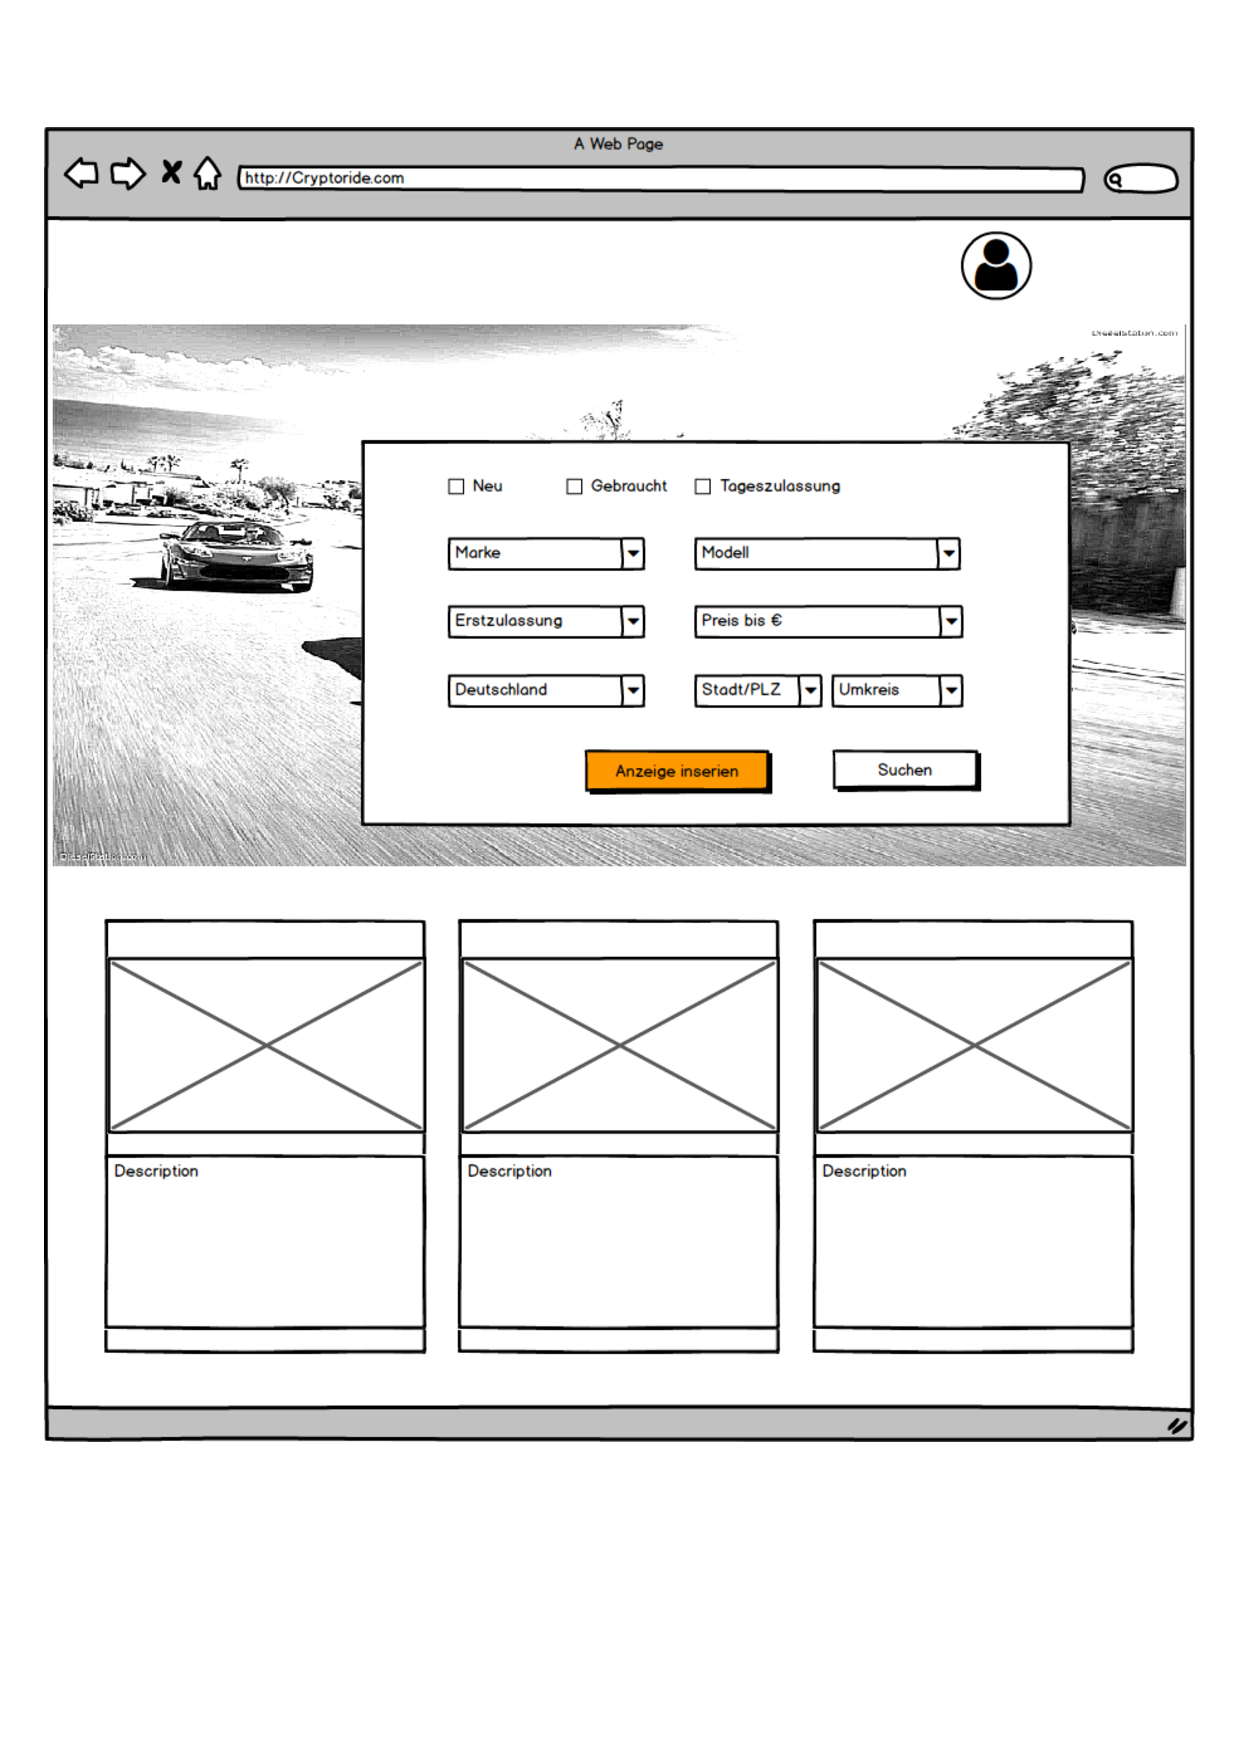
\includegraphics[width=0.9\textwidth]{figures/mockup_screen_01.pdf}}
\caption{Mockup of the home screen \label{fig:mockup_01}}
\end{figure}

\begin{figure}[htbp]
\centerline{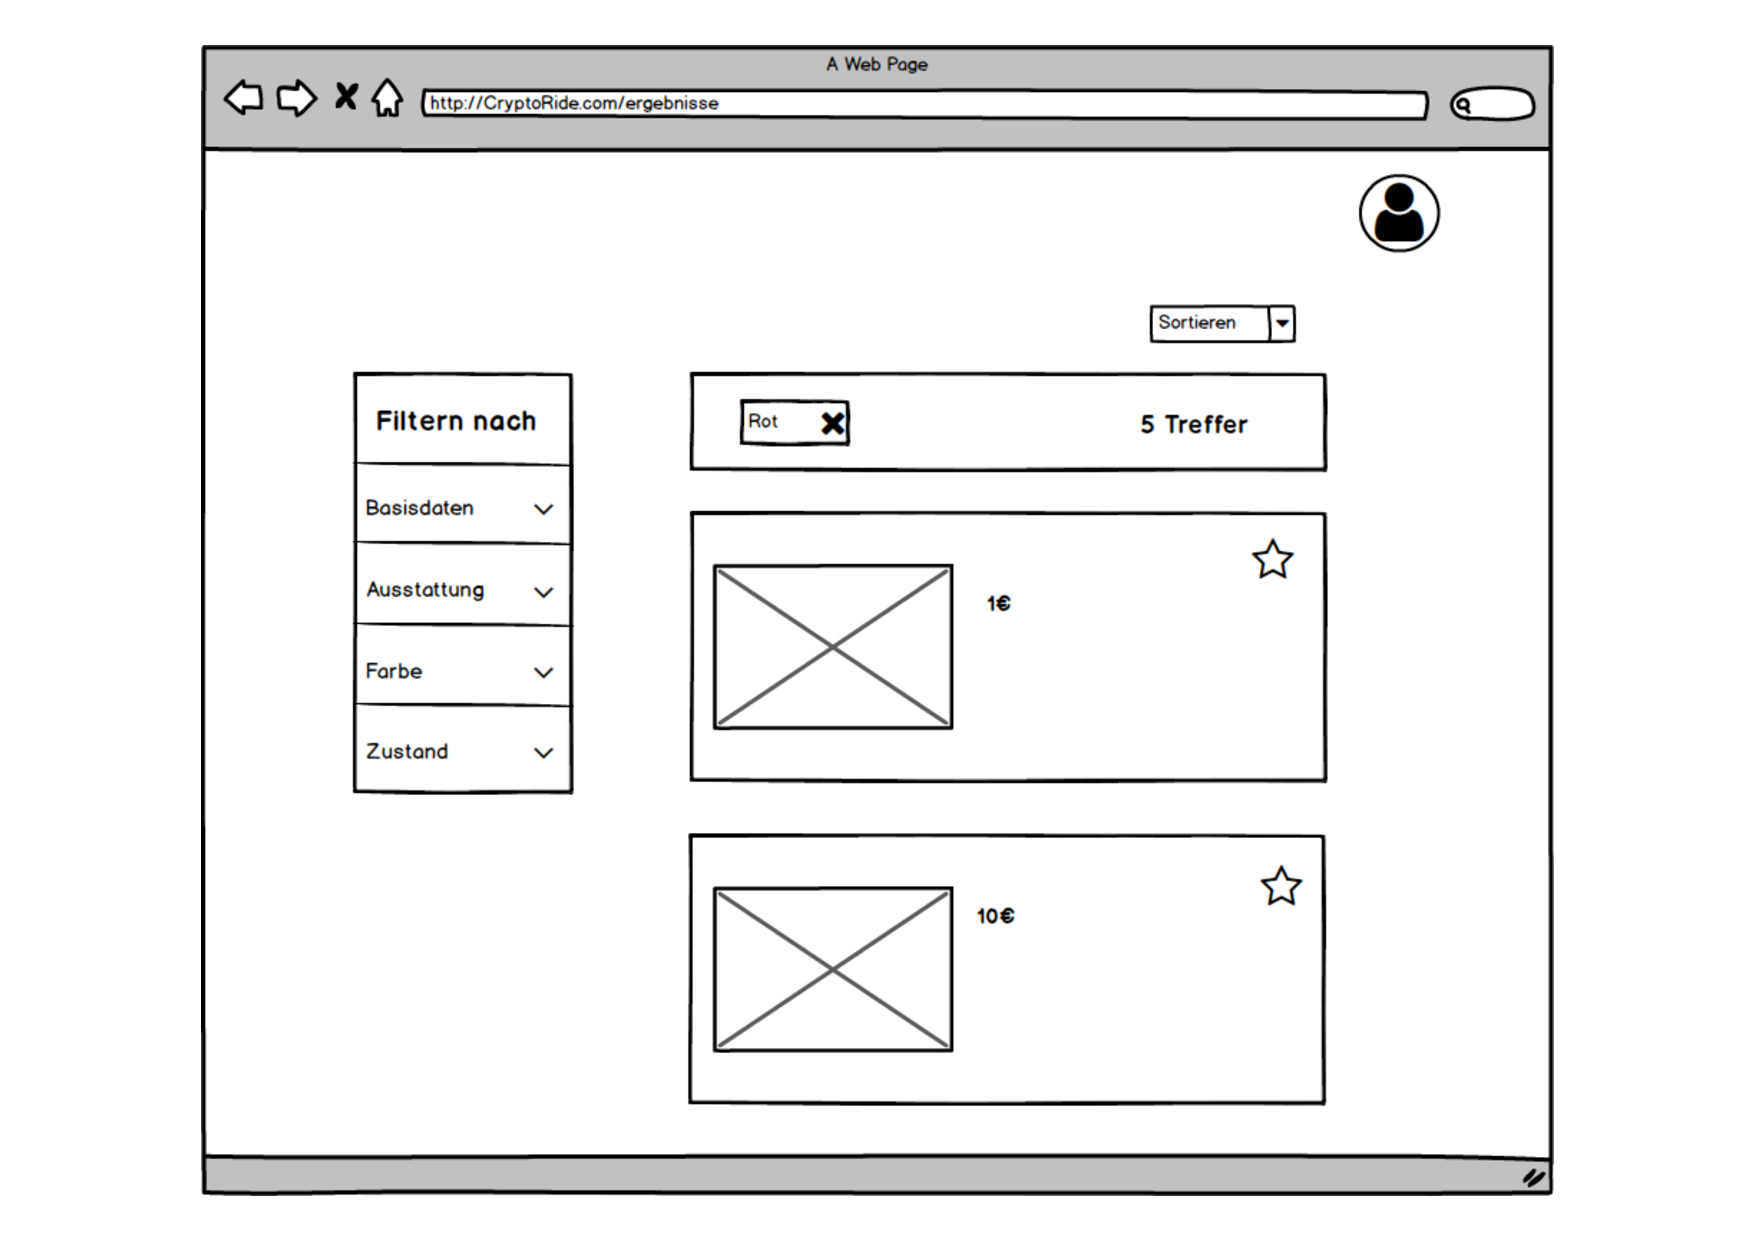
\includegraphics[width=0.9\textwidth]{figures/mockup_screen_02.pdf}}
\caption{Mockup of the search result screen \label{fig:mockup_02}}
\end{figure}


\subsection{Assumptions}\label{concept:assumptions}

Our approach is based on some assumptions regarding the car ecosystem. This includes car manufacturing, as well as compliance visits and mileage logging. At the current state, our approach would not be possible to implement in a way that it could provide the desired advantages mentioned in Section~\ref{sec:selling_points}. However, we do believe that adoption of blockchain technologies will eventually rise over the upcoming years.

Therefore, we assume in our scenario that car manufacturers already leverage blockchain technology. In specific, we make the following two assumptions. Firstly, when a car manufacturer produces a new car, it stores the car's identity on a blockchain which can be accessed by third-parties on demand. However, only car manufacturers are able to create a car on the blockchain. Secondly, we assume that new cars will be built in a way that enables them to store and update, on a regular basis, some of their key information, such as mileage, on a blockchain. Alternatively or additionally to the second point, we assume that trusted third-parties would be allowed to update details of a car, e.g the number of accidents, on the blockchain.

\clearpage
\section{Implementation} \label{sec:impl}
In this section, we will describe the implementation of our protype in detail. First, we will outline the used framework and tools in each application stack. Then, we will describe our development setup using Ethereum test network. Furthermore, we will describe the implementation of the core data structures and smart contracts. And finally, we will explain the secured transaction flow without a need for a trusted third-party.

\subsection{Architecture}
Our technology stack is illustrated in Figure~\ref{fig:techstack}. For the web front-end we used the popular setup containing React~\cite{React}, Webpack~\cite{Webpack} and Redux~\cite{Redux} using JavaScript as the primary programming language. The smart contracts are written in Solidity. Additionally, we utilized various tools such as Truffle~\cite{Truffle}, a widely-used development framework for Ethereum. Although Truffle allows us to run a local Ethereum testnet, Ganache~\cite{Ganache} came in very handy since it offered an user interface, where we could inspect the current state of the ledger including all performed transactions. Additionally, we used OpenZeppelin~\cite{OpenZeppelin}, a framework containing reusable smart contracts (e.g. access control, ERC-20, ERC-721, ...) that have been tested and reviewed by the Ethereum community. As for the backend, we went with Node.js using ExpressJS as the underlying web-framework along with MongoDB to persist meta-data of car assets and sales.

\begin{figure}[htbp]
\centerline{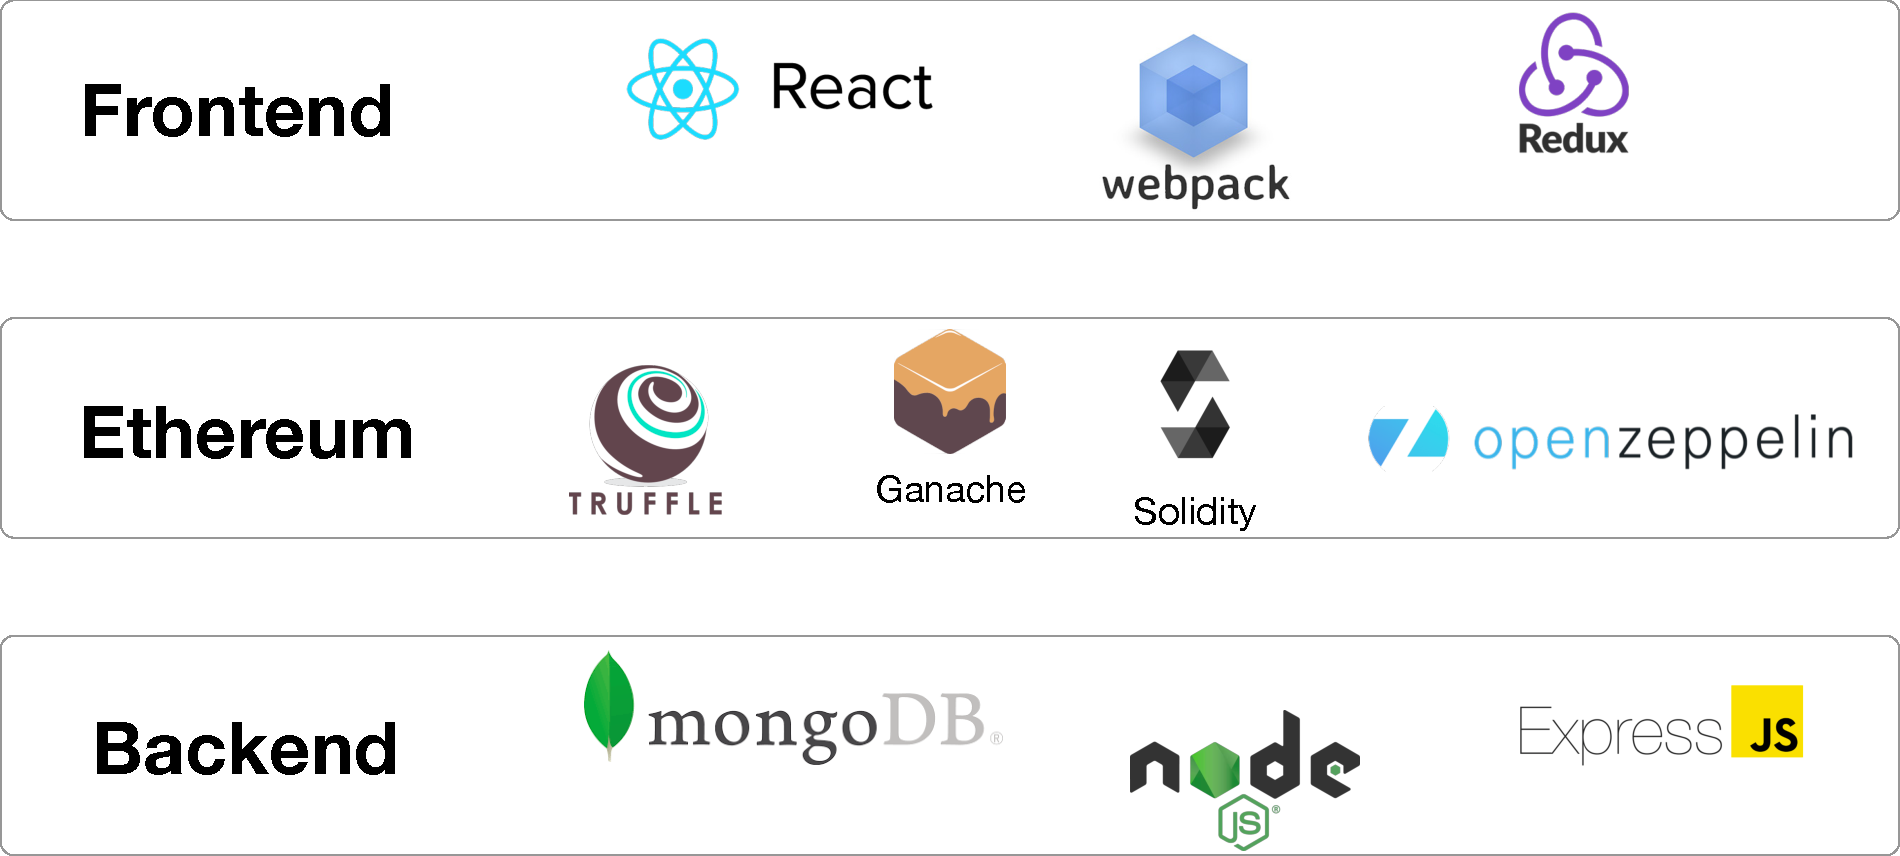
\includegraphics[width=0.9\textwidth]{figures/tech_stack.pdf}}
\caption{Technology stack \label{fig:techstack}}
\end{figure}

\subsection{Ethereum Test Network}
For deploying and testing our smart contracts, we used a personal blockchain which only runs on our system and does not interact with the main Ethereum network. Truffle's command line interface allows such setup which comes with ten Ethereum wallets containing 100 Ether each. This allows us to test smart contracts freely without paying real fees. An alternative would be deploying the smart contracts to one of the many testnets (e.g. Rinkeby~\cite{Rinkeby}) which allows a better testing of the real world performance. This is especially useful when nearing production stage, however before that, we found it to be too inconvenient, tedious which slows down the development tremendously.

\subsection{Data Structures}
In order to store car assets and make them temper-proof, we had to define the corresponding data structures that are stored and managed directly on the Ethereum ledger. The struct as shown in Listing~\ref{lst:car_struct} represents a car, it contains only the most important attributes such as manufacturer, mileage and accidents count. Note that we decided against storing additional attributes, because persisting large amount of data on Ethereum can be very costly and could lead to blockchain bloating~\cite{BlockchainBloating}. Instead, non-critical information (e.g. horse power, images) are stored in our back-end database. Since cars are not removable, they are all stored in an growing array, where the array index also serves as the car identifier. Sale structures also only contain the most important information: seller, bidder, price of the car and time when the sale has started (see Listing~\ref{lst:sale_struct}). Unlike cars, sales are stored inside a mapping with the asset identifer as the key value. This allows the deletion of a sale after it has been finished.

\begin{minipage}[t]{0.45\linewidth}
\begin{lstlisting}[caption={Car struct}, language=Solidity, label=lst:car_struct, numbers=none]
struct Car {

  // The timestamp of car creation.
  uint64 creationTime;

  // The ID of the car manufacturer
  uint256 manufacturerId;

  // The ID of the car model
  uint16 modelId;

  // The mileage of the car (in km)
  uint32 mileage;

  // Number of accidents involving this car
  uint8 accidentsCount;
}
\end{lstlisting}
\end{minipage}
\hspace{10mm}
\begin{minipage}[t]{0.45\linewidth}
\begin{lstlisting}[caption={Sale struct}, language=Solidity, label=lst:sale_struct, numbers=none]
struct Sale {
  // Current car owner
  address seller;
  // Person who has bid on this sale
  address bidder;
  // Car Price
  uint128 price;
  // Time when sale started
  uint64 startedAt;
}
\end{lstlisting}
\end{minipage}

\clearpage

\subsection{Smart Contracts}
An overview of the smart contracts is shown in Figure~\ref{fig:class_diagram}.
We split the various functionalities in different contracts and used inheritance to combine them meaningfully. Effectively, the application consists of two main contracts which we will describe in the following more in detail.

\subsubsection{Access Control}
As mentioned in our concept (see Section ~\ref{sec:concept}), the creation and update of cars is only permitted to car manufacturers. Therefor, we implemented an access control mechanism, which contains the following two roles:
  \begin{enumerate}
    \item \textbf{Administrator}: can add or remove manufacturers
    \item \textbf{Manufacturer}: can initially create car assets and update car statistics (e.g. mileage)
  \end{enumerate}
To achieve this, our implementation inherits from OpenZeppelin's role-based access control (RBAC) smart contracts~\cite{OpenZeppelinGithub}.

\subsubsection{Car}
The \textit{RideBase} contract serves as the foundation for our DApp, it holds all common structs, events and variables. In particular, it defines the array containing all car structs and a mapping of car identifiers to their owners. Additionally, it holds a reference to our market contract, allowing the interaction with it. This reference can be updated after deployment so that we can replace the market contract in case something goes wrong. The \textit{RideCore} contract is the main interface for interacting with our DApp, is handles creating, updating and tracking the current status of cars.

\subsubsection{Ownership}
Tracking and transferring the ownership of an asset is a well-known use case in blockchain technology. Fortunately, the ERC-721 Non-Fungible Token Standard~\cite{ERC721Summary} provides a solution for this (see also Section~\ref{sec:ERC721}). Non-fungible tokens (NFTs) can represent ownership over digital or physical assets such as houses, collectable cards but also cars. NFTs are unique, distinguishable and are thus not interchangeable. The \textit{RideOwnership} contract, from which our main car contract inherits from, implements the ERC-721 interface. By utilizing the mapping from asset identifier to owner address, we can always ensure the correctness of asset ownership and transfer.

\subsubsection{Market}
Our market implementation consists of two contracts. The first is \textit{MarketBase} which contains all structs, events, and internal methods for managing sales. In particular, it holds a mapping of assets to their corresponding sale structs and a reference to the ERC-271 implementation to perform ownership transfers. The second contract is \textit{MarketCore} which inherits from \textit{MarketBase} and provides the main interface for interacting with the sales. It handles operations such as creating sales, tracking the current status of sales, bidding on sales, confirming or rejecting sales.

\subsection{Transaction Flow}
In order to make the transaction between buyer and seller trustless and secure, we implemented an escrow mechanism which should simulate the intermediary third-party. Only upon certain conditions, the ownership transfer is performed. In the first iteration, we implemented the transaction process like the following:
\begin{enumerate}
  \item \textbf{Sell}: Seller defines a price and puts a car on sale. I.e. car asset is transferred to our market contract.
  \item \textbf{Buy}: Buyer pays the requested price, the money goes to our market contract.
  \item \textbf{Escrow}: Car is transferred to buyer and the money is transferred to seller simultaneously.
\end{enumerate}

Although this approach works in theory, there are several flaws that made us rethink the whole process. Firstly, the seller cannot really decide to whom the car is sold, since it is basically first come, first served. Secondly, once the transaction is performed, there is no way for the buyer to cancel his order, since it automatically goes through if the requested price was paid. For this particular reasons, we updated the flow and added an extra confirmation step.

\begin{enumerate}
    \item \textbf{Sell}: Seller defines a price and puts a car on sale. I.e. car asset is transferred to our market contract.
    \item \textbf{Bid}: Buyer bids on car and pays the requested price upfront, the money goes to our market contract. Car is now reserved, meaning no other person can place a new bid on it.
    \item \textbf{Confirm}: Buyer and seller both now have the option to cancel the bid, thus returning the money back to the buyer and make the car available again. Seller has additional option to confirm the bid which triggers the asset transfer.
    \item \textbf{Escrow}: If confirmed, car is transferred to buyer and the money is transferred to seller simultaneously.
  \end{enumerate}

This extra step should mitigate human errors and give buyer and seller more room for action. In addition to that, it improves the resemblance to the real world process of buying a car.

\begin{figure}[htbp]
\centerline{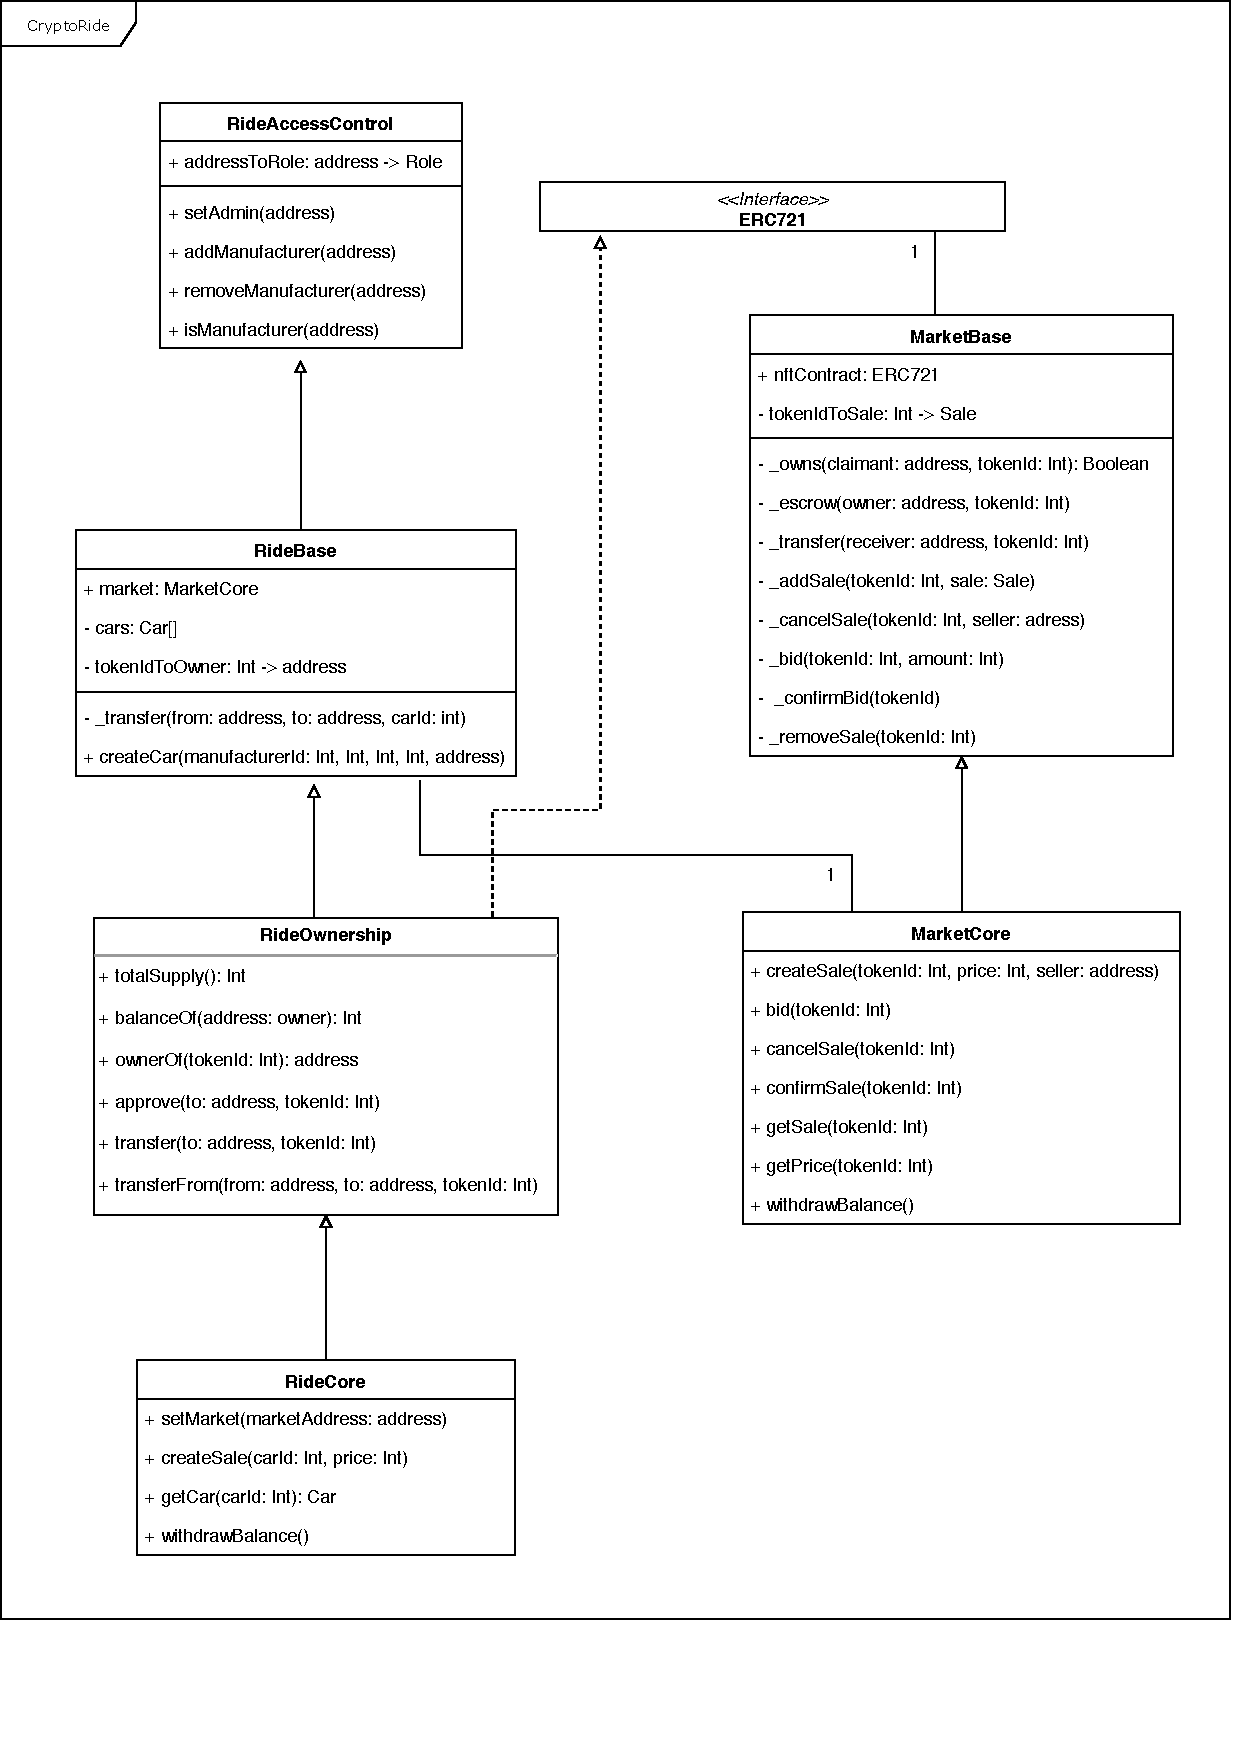
\includegraphics[width=\textwidth,height=\textheight,keepaspectratio]{figures/smart_contracts_uml.pdf}}
\caption{Overview: Smart Contracts \label{fig:class_diagram}}
\end{figure}


% \subsubsection{Testing}
% In order to verify the correctness and functional behavior of our smart contracts, we implemented automated tests, which should simulate the user interactions with our application (e.g. creating a car, selling and buying a car, etc.). The tests are written in Solidity or JavaScript and are executed using Truffle's command line interface~\cite{TruffleTest}.

\clearpage

\subsection{MetaMask}
MetaMask~\cite{MetaMask} is an extension which allows users to interact with the Ethereum network directly from the browser. It serves as our main tool for the secure user authentication and car asset transfer. By injecting the Ethereum web3 API into every website's JavaScript context, DApps can read from the blockchain through MetaMask. Furthermore, it lets users create and manage their identities, i.e. when a DApp wants to perform a transaction, the user is notified with a secure interface for reviewing the transaction before accepting or rejecting it (see Figure~\ref{fig:metamask_transaction}). In order to interact with our application, the MetaMask browser extension has to be installed either on Google Chrome or Mozilla Firefox.

\begin{figure}[htb]
  \centering
  \begin{subfigure}{.4\textwidth}
    \centering
    \fbox{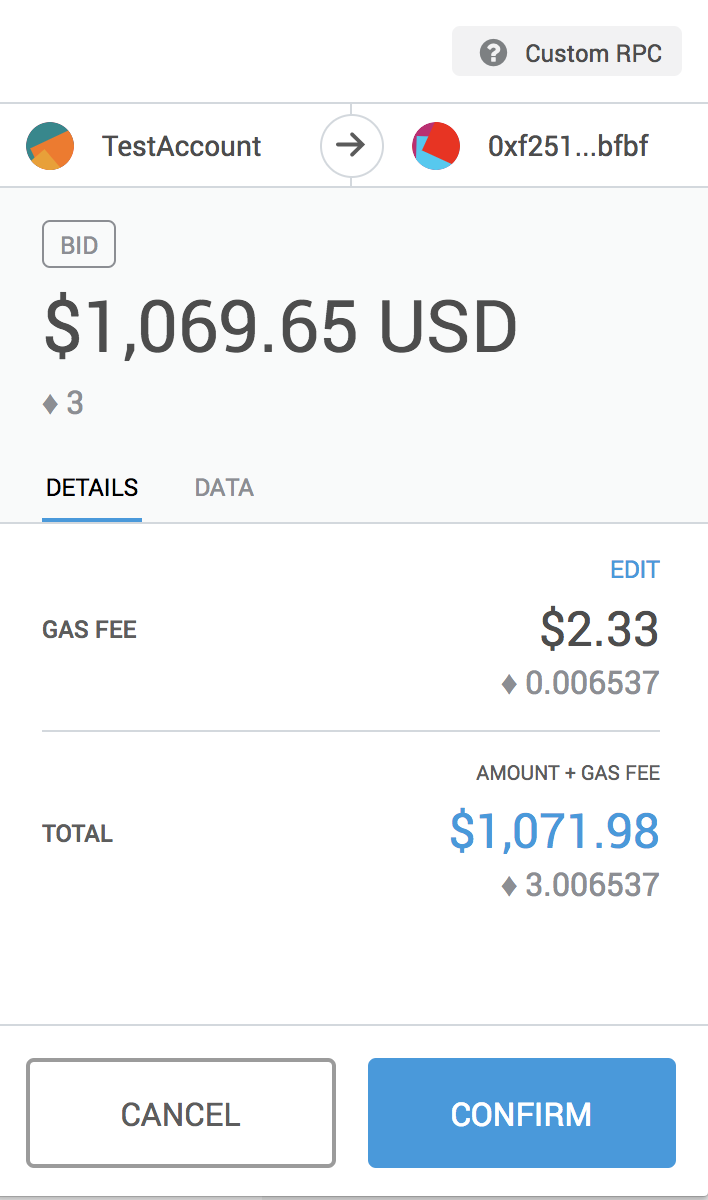
\includegraphics[width=0.9\linewidth]{figures/cryptoride_screens/metamask_transaction.png}}
    \caption{Transaction \label{fig:metamask_transaction}}
  \end{subfigure}
  \hspace{10mm}
  \begin{subfigure}{.4\textwidth}
    \centering
    \fbox{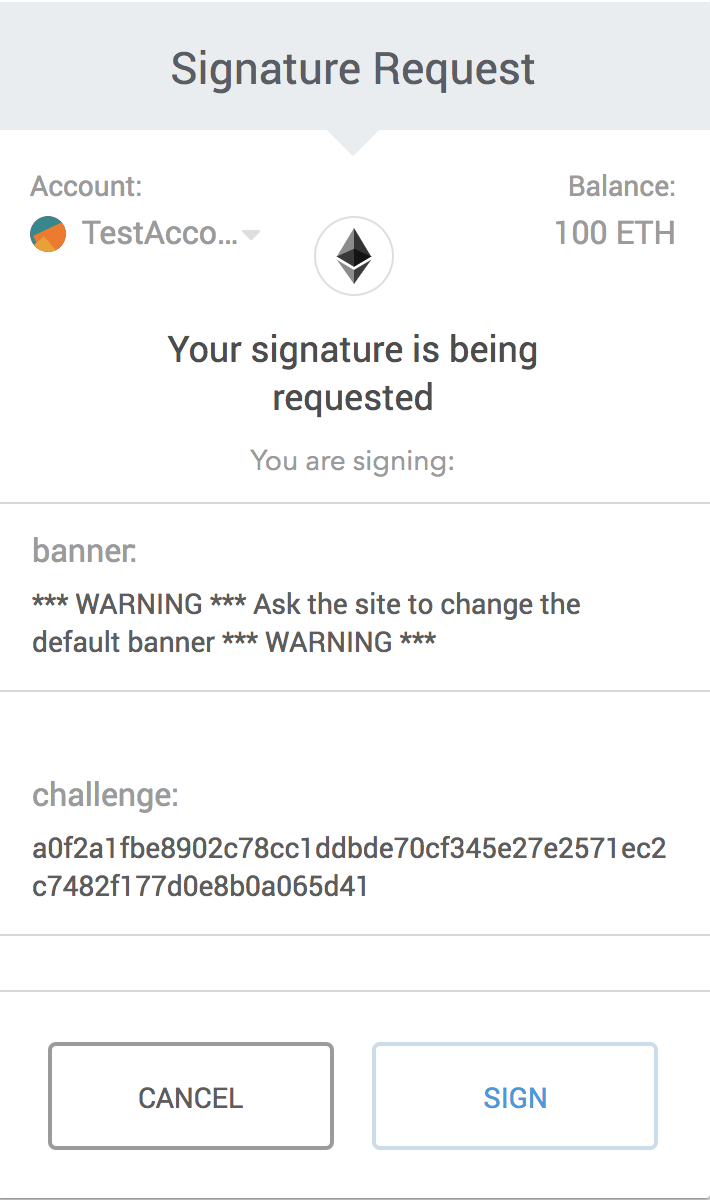
\includegraphics[width=0.9\linewidth]{figures/cryptoride_screens/metamask_sign.png}}
    \caption{Signing \label{fig:metamask_signing}}
  \end{subfigure}
  \caption{MetaMask}
\end{figure}


% \subsection{Application Flow}
% A rough overview of the application flow is illustrated in Figure~\ref{fig:application_flow}. In order to use our platform, an account is needed. This can be done by registrating with a valid Ethereum account and having MetaMask installed on the browser. When logged in, the user can look for active sales or putting a car on sale. Manufacturers addresses are recognized by the front-end, they are permitted to create new car assets.

\subsubsection{Authentication}
We use MetaMask for handling user authentication over the traditional username and password login. This approach only requires an Ethereum account and no personal identifying information.
First, the user is asked to sign a challenge using his private key (see Figure~\ref{fig:metamask_signing}). Then, the generated signature is then sent to the back-end for validation. Finally, upon success, the backend will respond with a JSON Web Token (JWT) which authenticates the user. This token can also be stored for the current session.

% \begin{figure}[htbp]
% \centerline{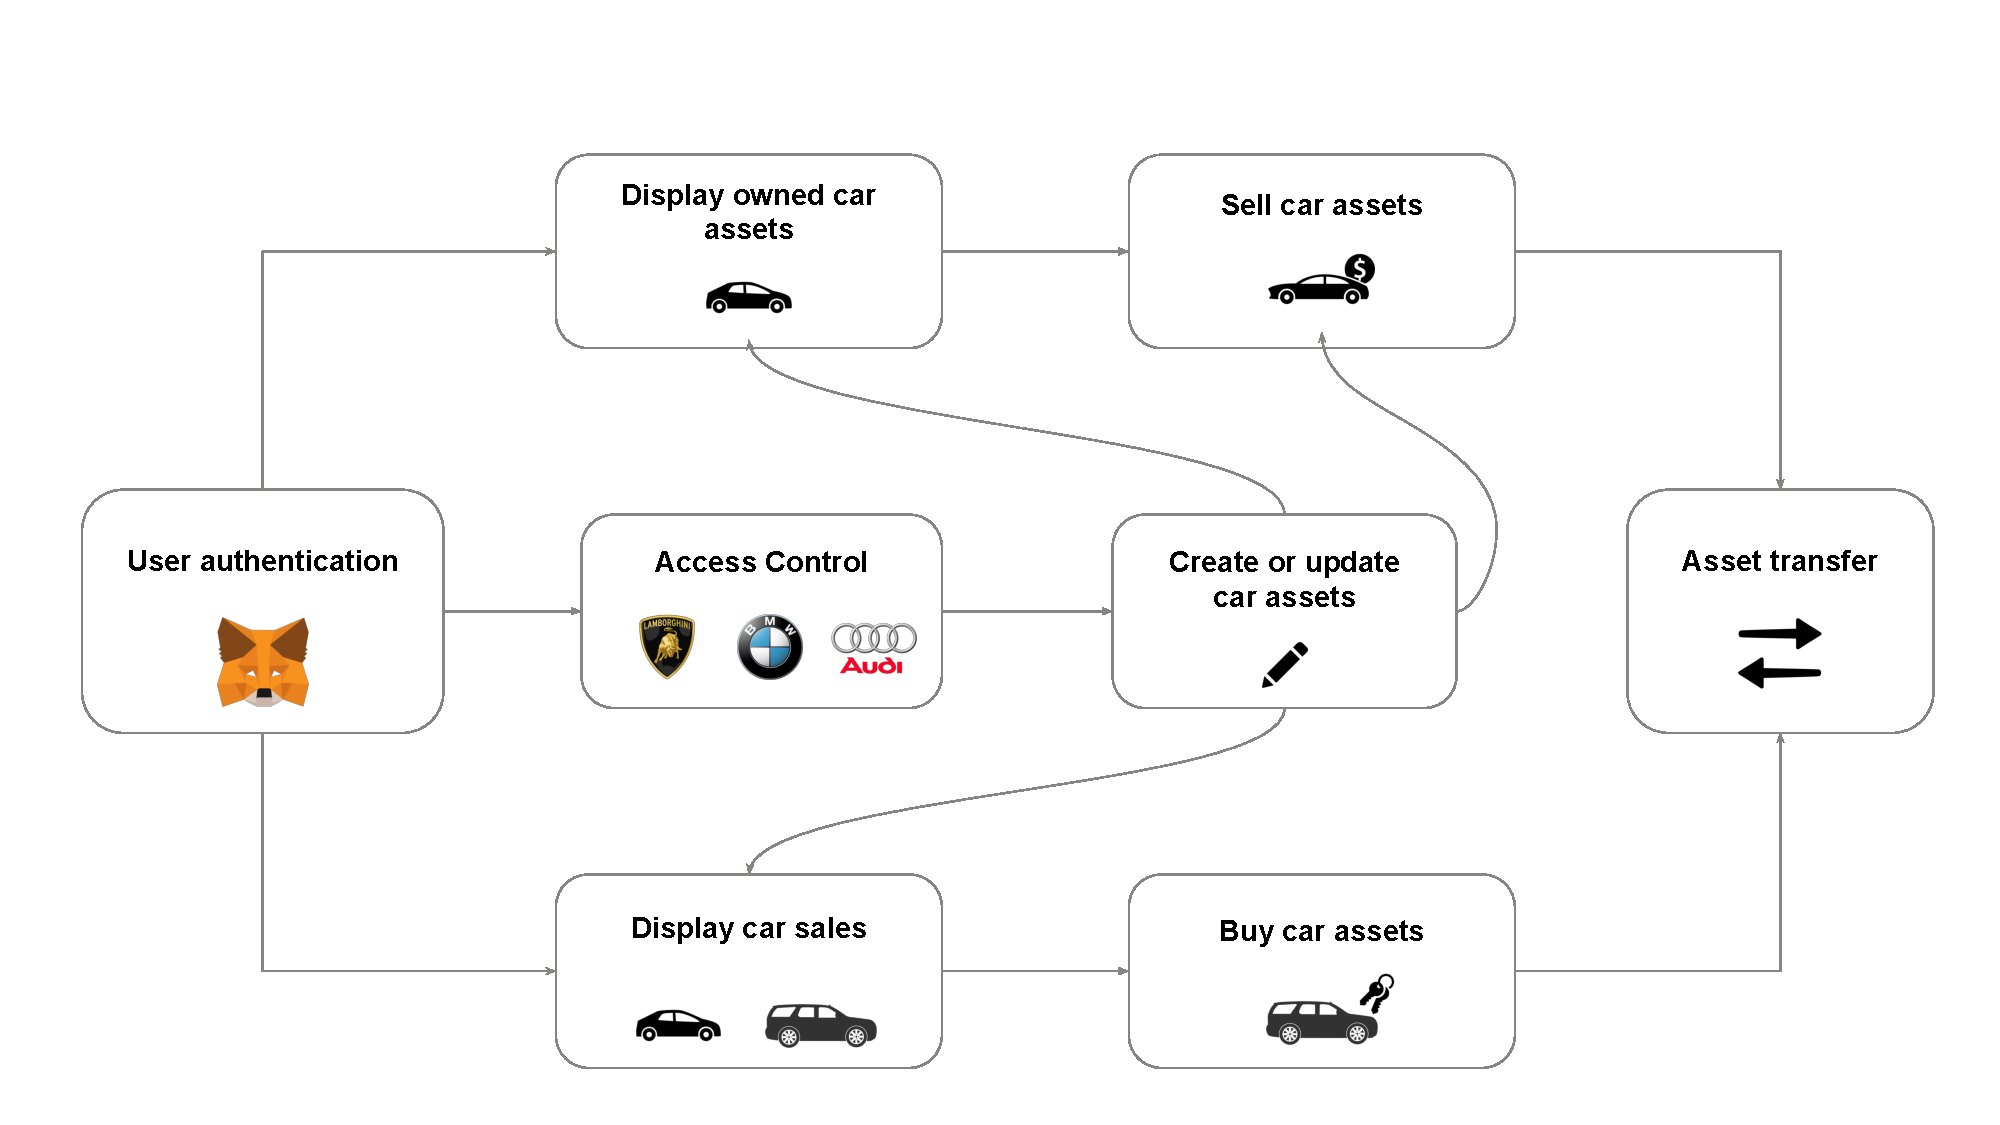
\includegraphics[width=0.9\textwidth]{figures/application_flow.pdf}}
% \caption{Application Flow \label{fig:application_flow}}
% \end{figure}



% \subsection{Screenshots}
% \begin{figure}[htbp]
% \centerline{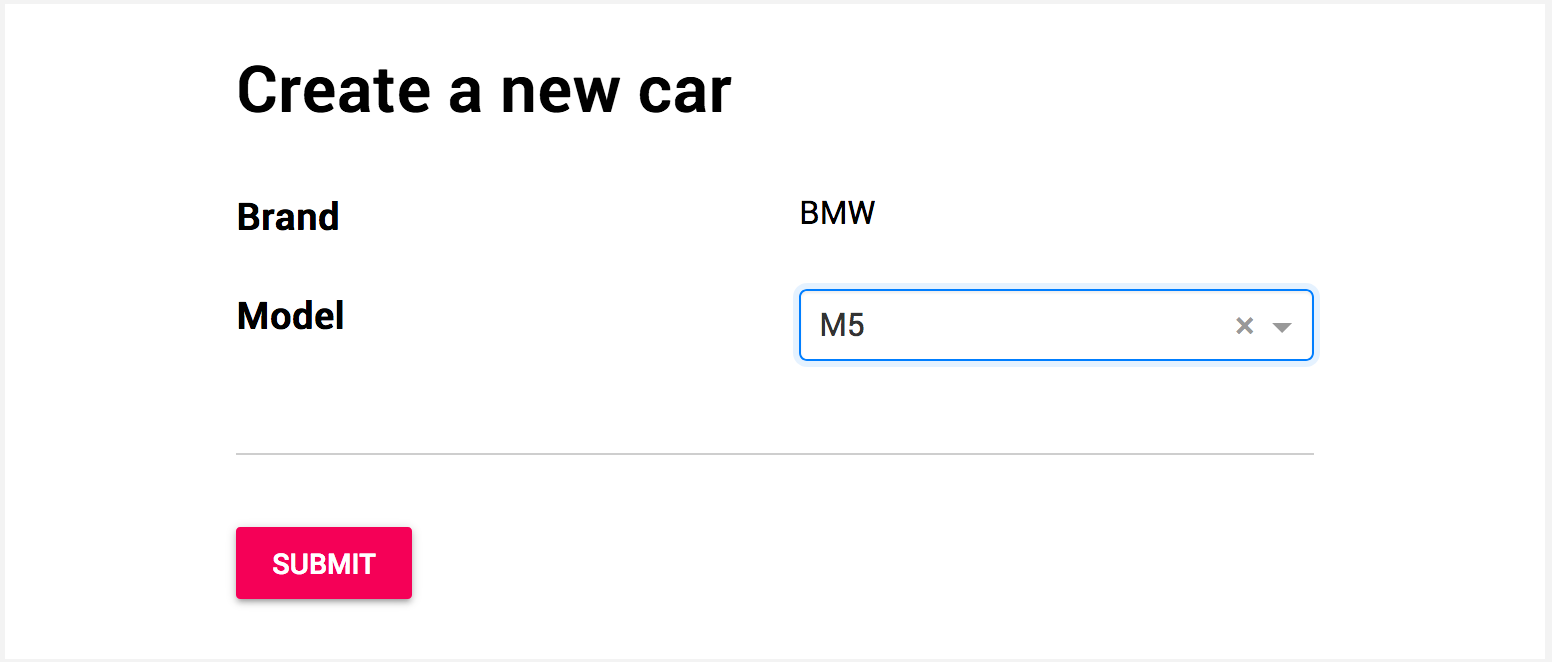
\includegraphics[width=1\textwidth]{figures/cryptoride_screens/create_car.png}}
% \caption{Screen: Create Car \label{fig:screen_create_car}}
% \end{figure}
%
% \begin{figure}[htbp]
% \centerline{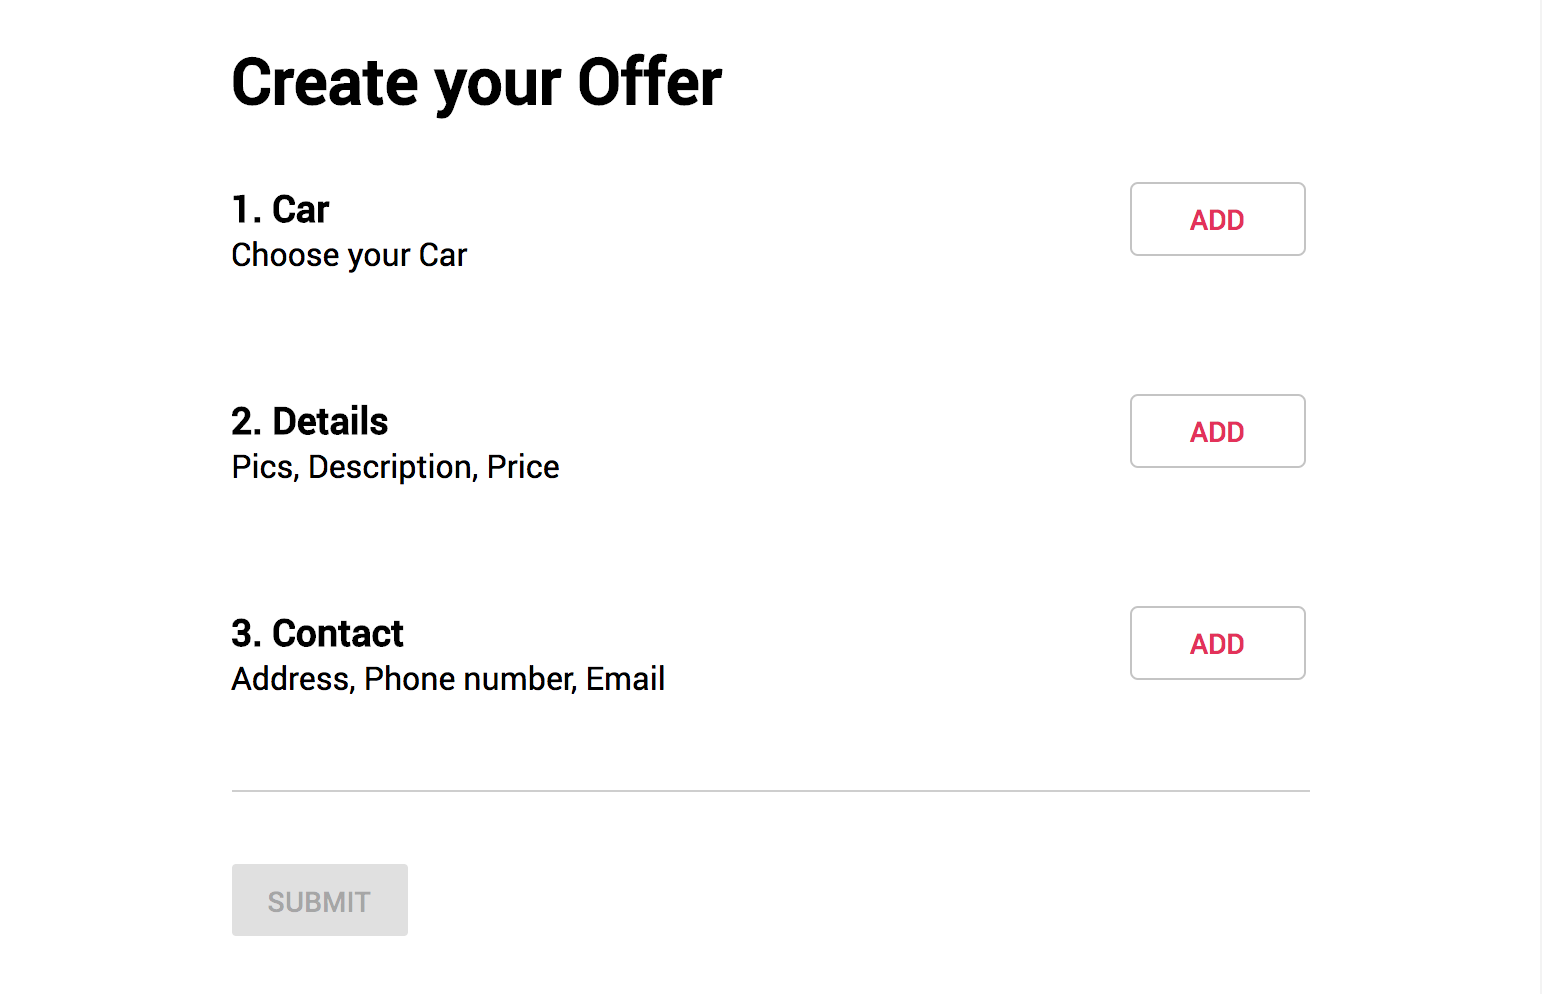
\includegraphics[width=1\textwidth]{figures/cryptoride_screens/create_offer.png}}
% \caption{Screen: Create Offer \label{fig:screen_create_offer}}
% \end{figure}
%
% \begin{figure}[htbp]
% \centerline{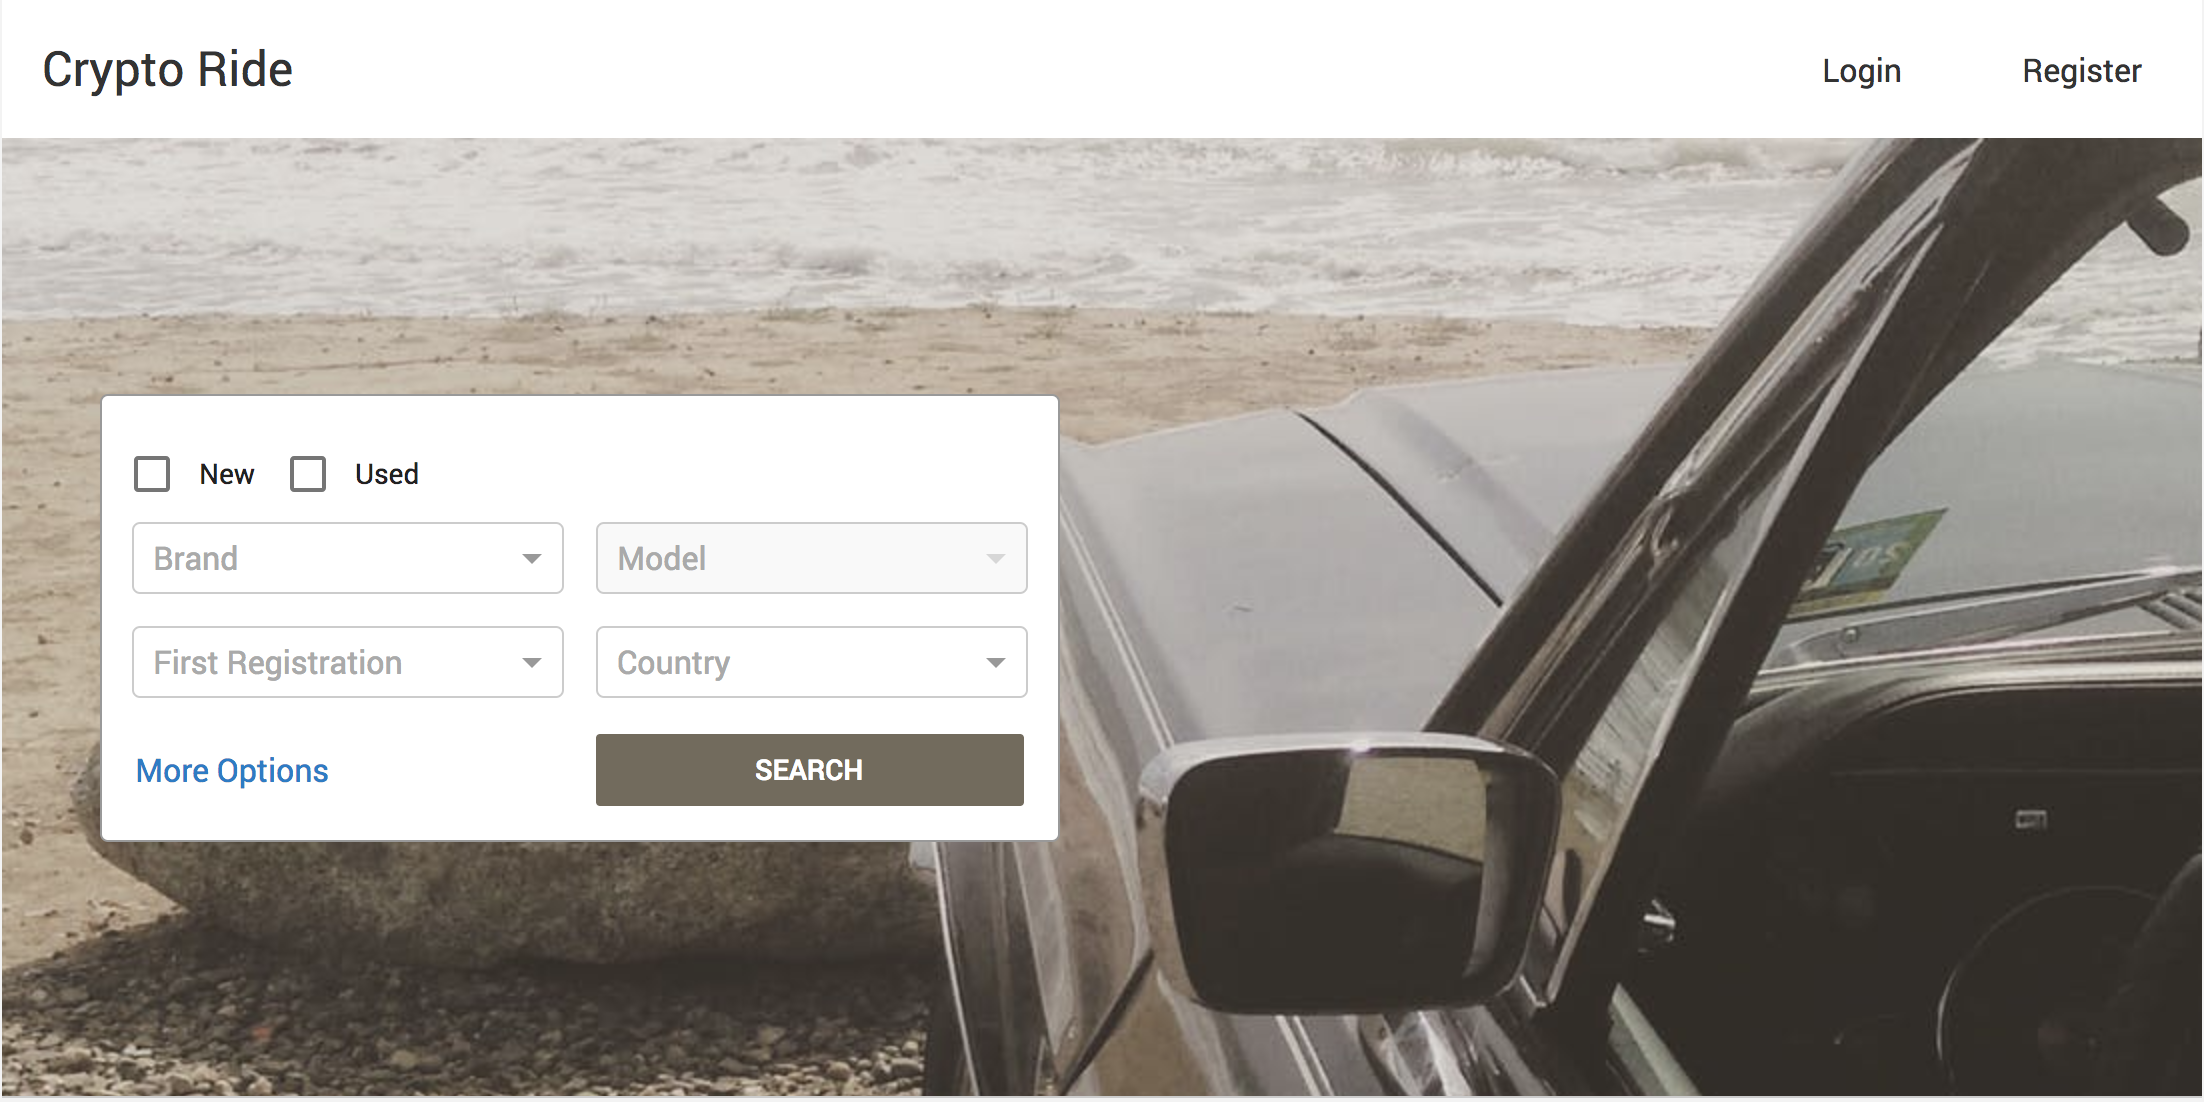
\includegraphics[width=1\textwidth]{figures/cryptoride_screens/cryptoride_landing_page.png}}
% \caption{Screen: Landing page \label{fig:screen_landing_page}}
% \end{figure}
%
%
% \begin{figure}[htbp]
% \centerline{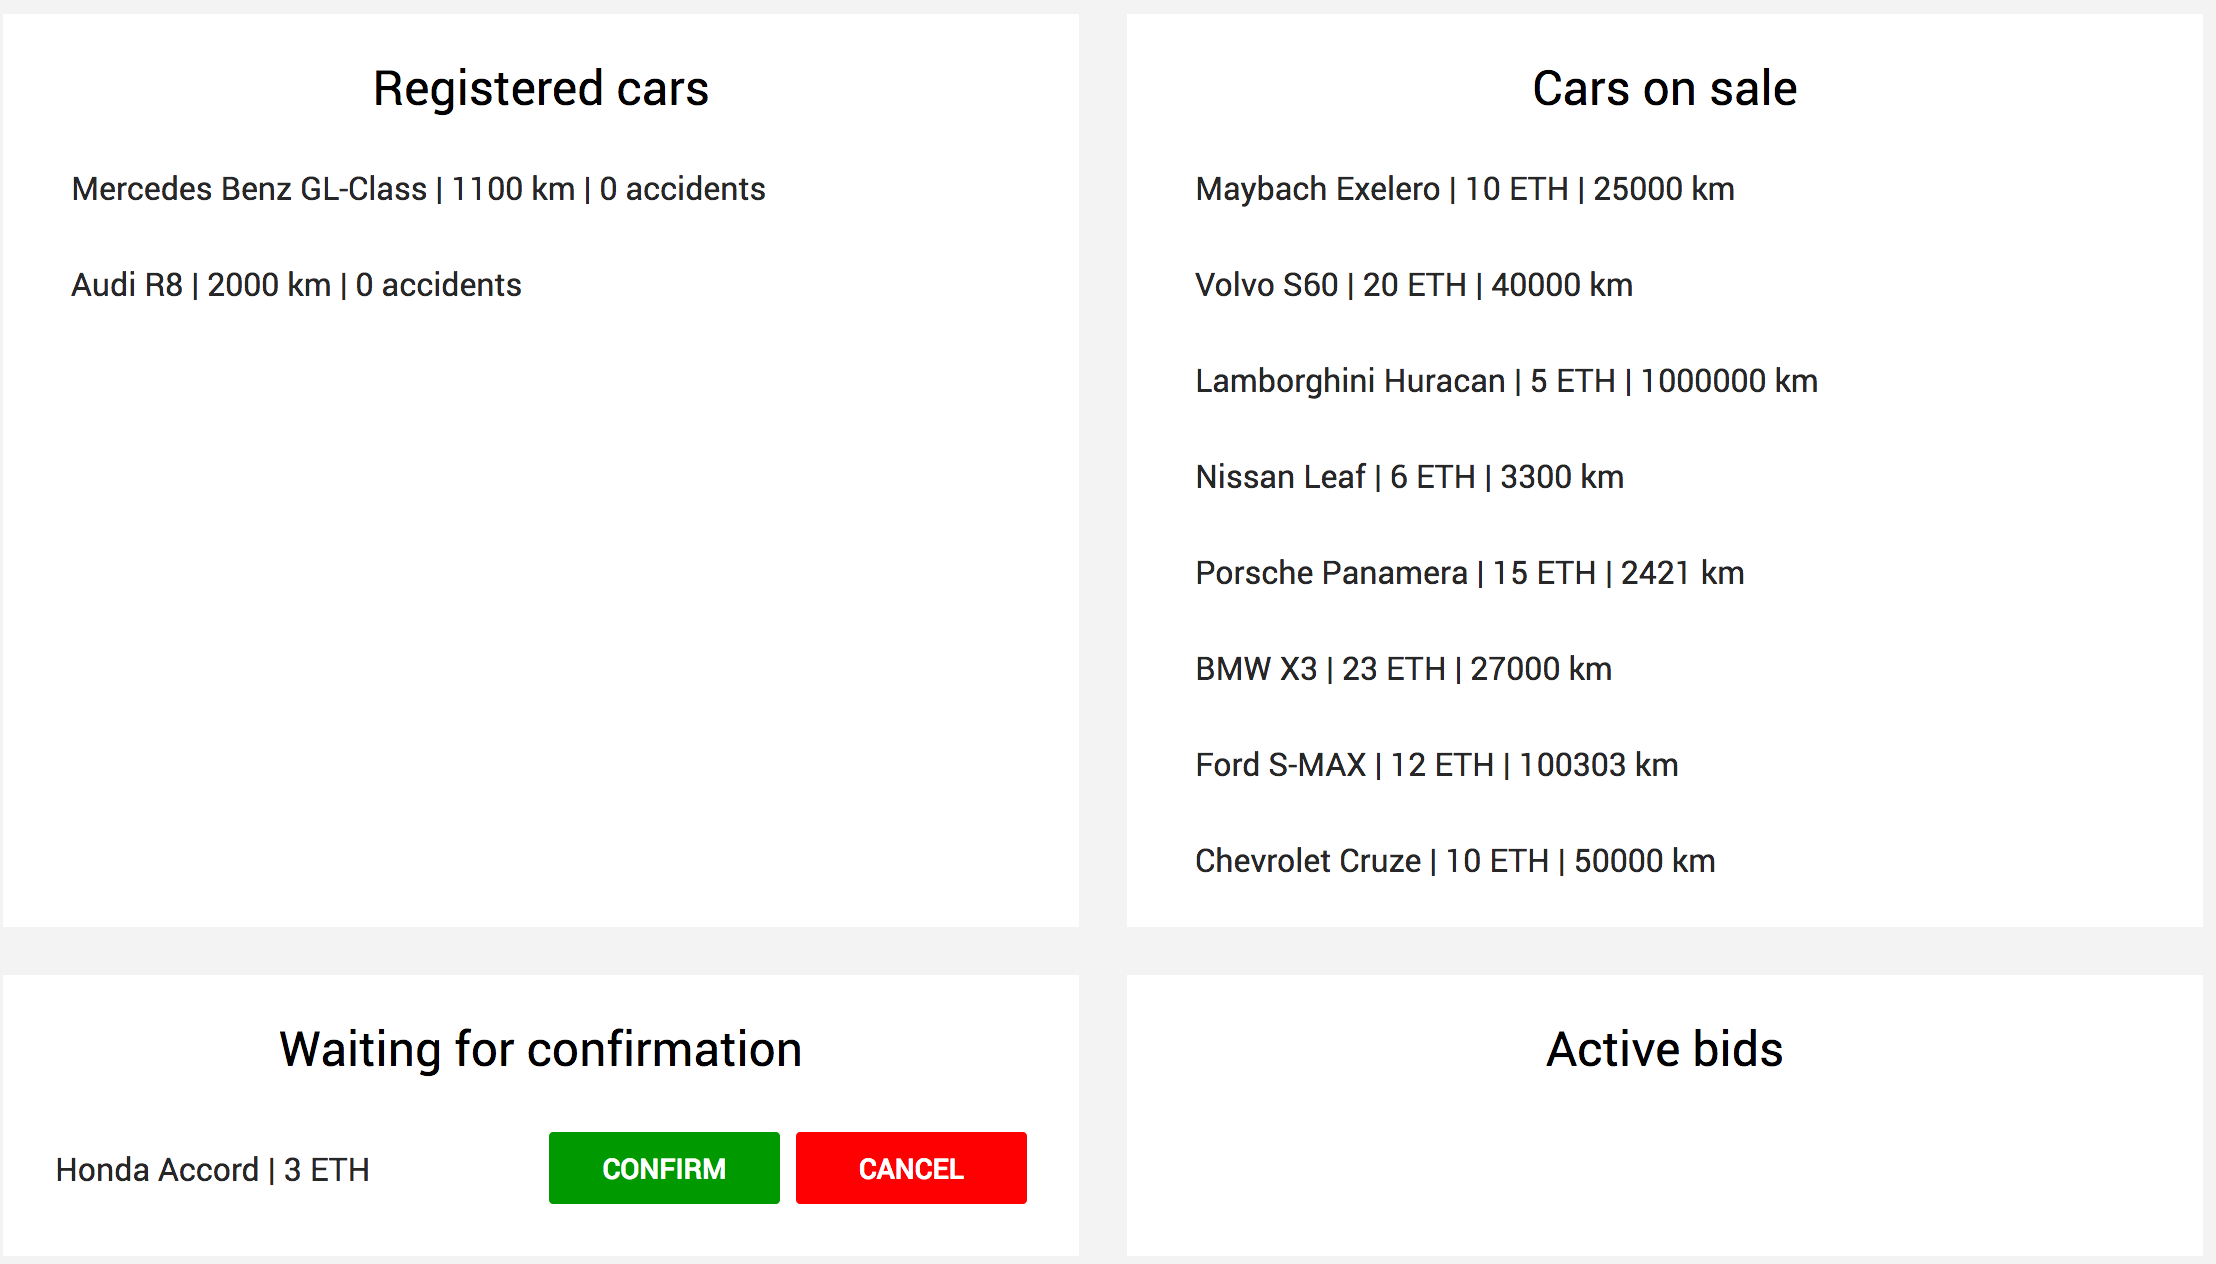
\includegraphics[width=1\textwidth]{figures/cryptoride_screens/my_cars.png}}
% \caption{Screen: My cars \label{fig:screen_my_cars}}
% \end{figure}
%
% \begin{figure}[htbp]
% \centerline{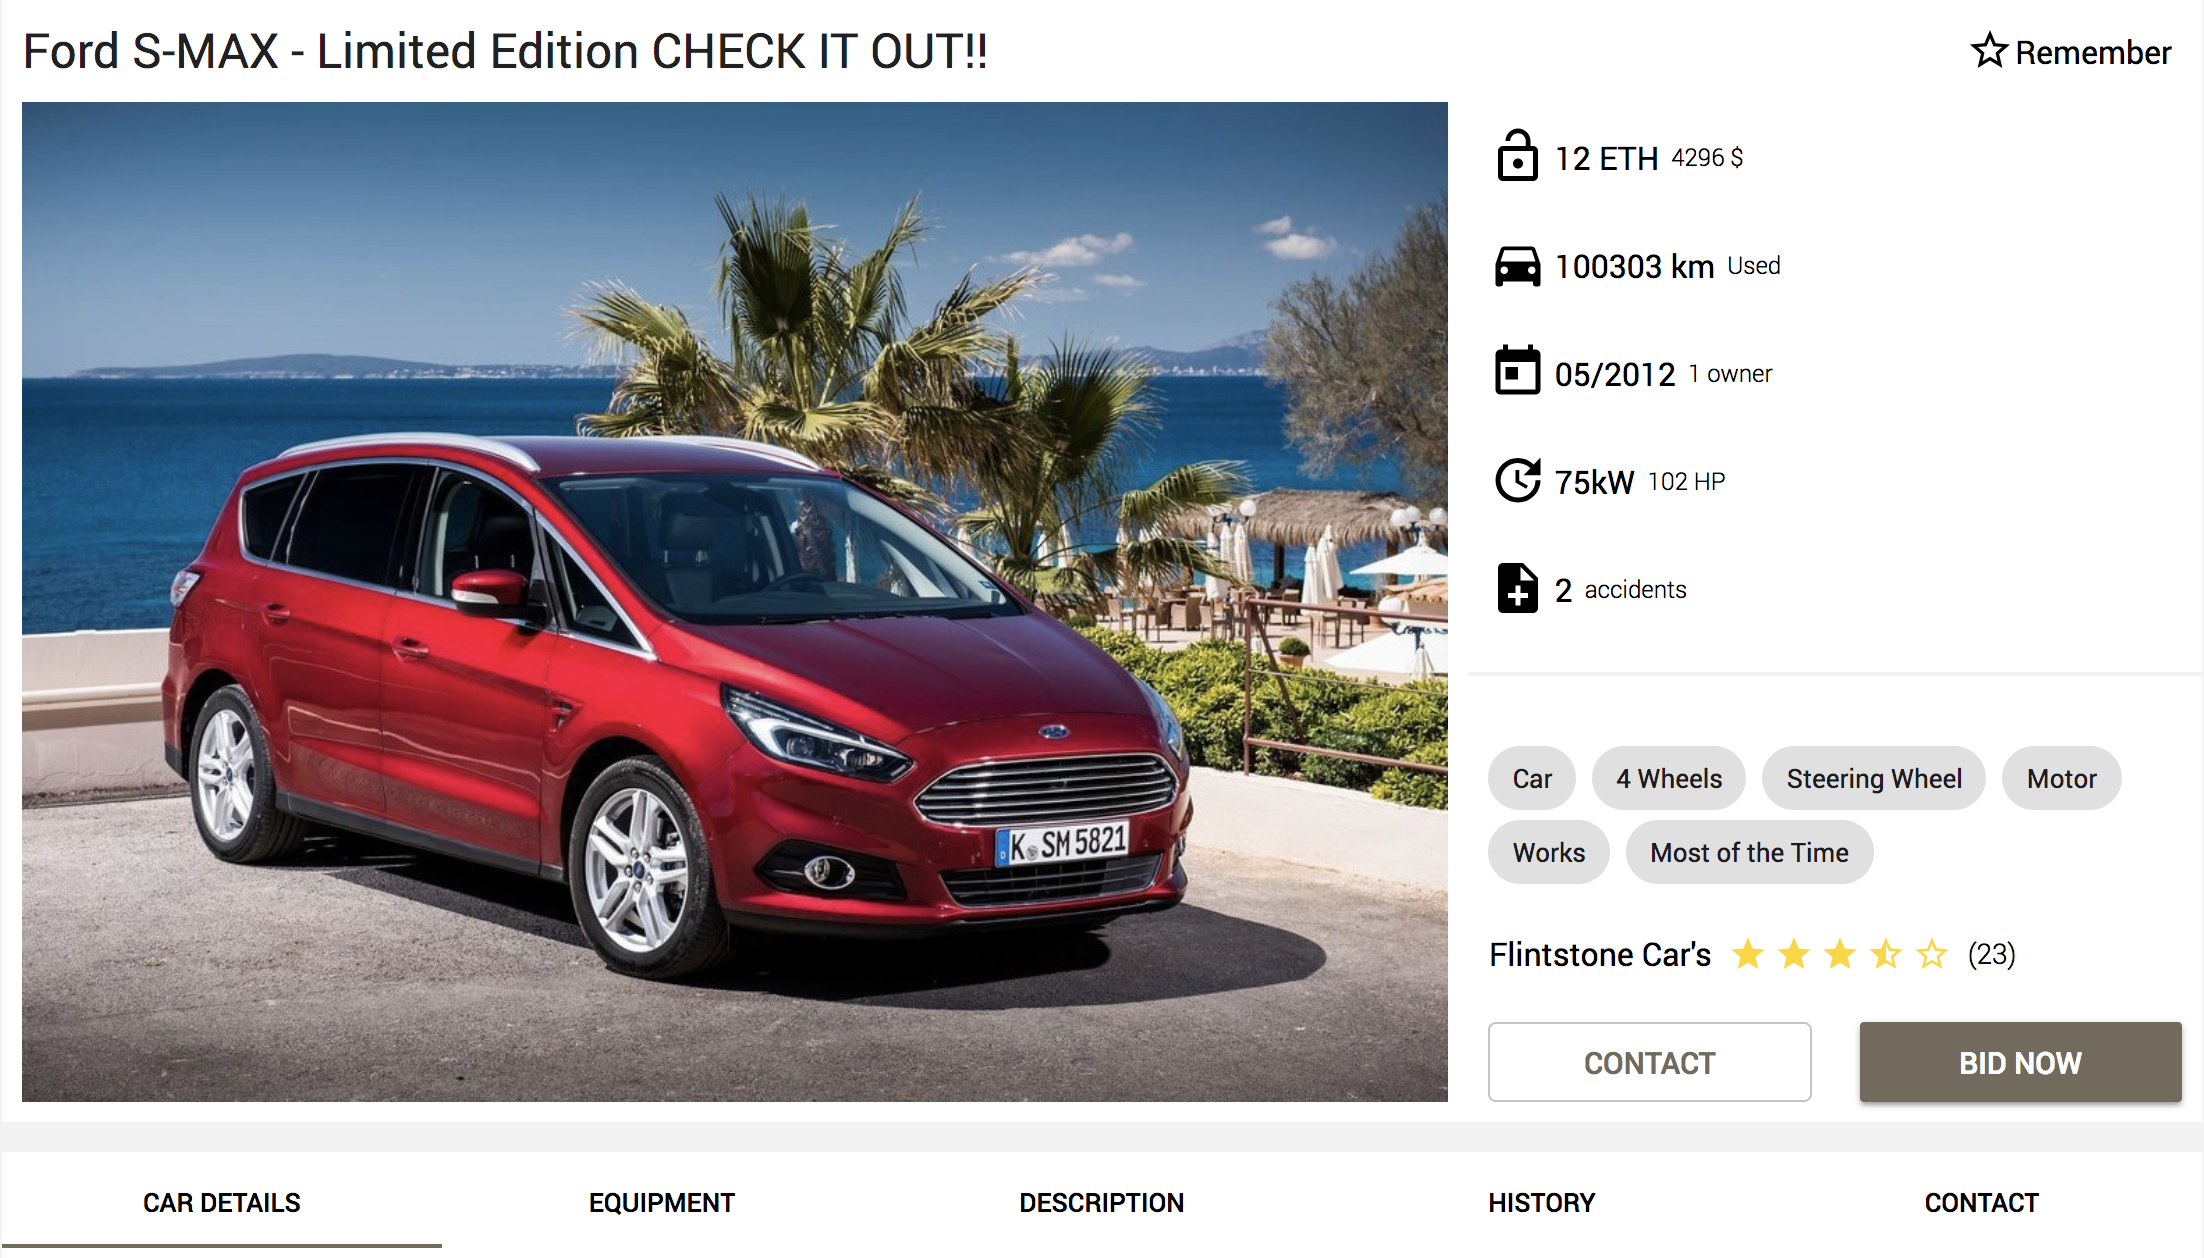
\includegraphics[width=1\textwidth]{figures/cryptoride_screens/offer_details.png}}
% \caption{Screen: Over details \label{fig:screen_offer_details}}
% \end{figure}
%
% \begin{figure}[htbp]
% \centerline{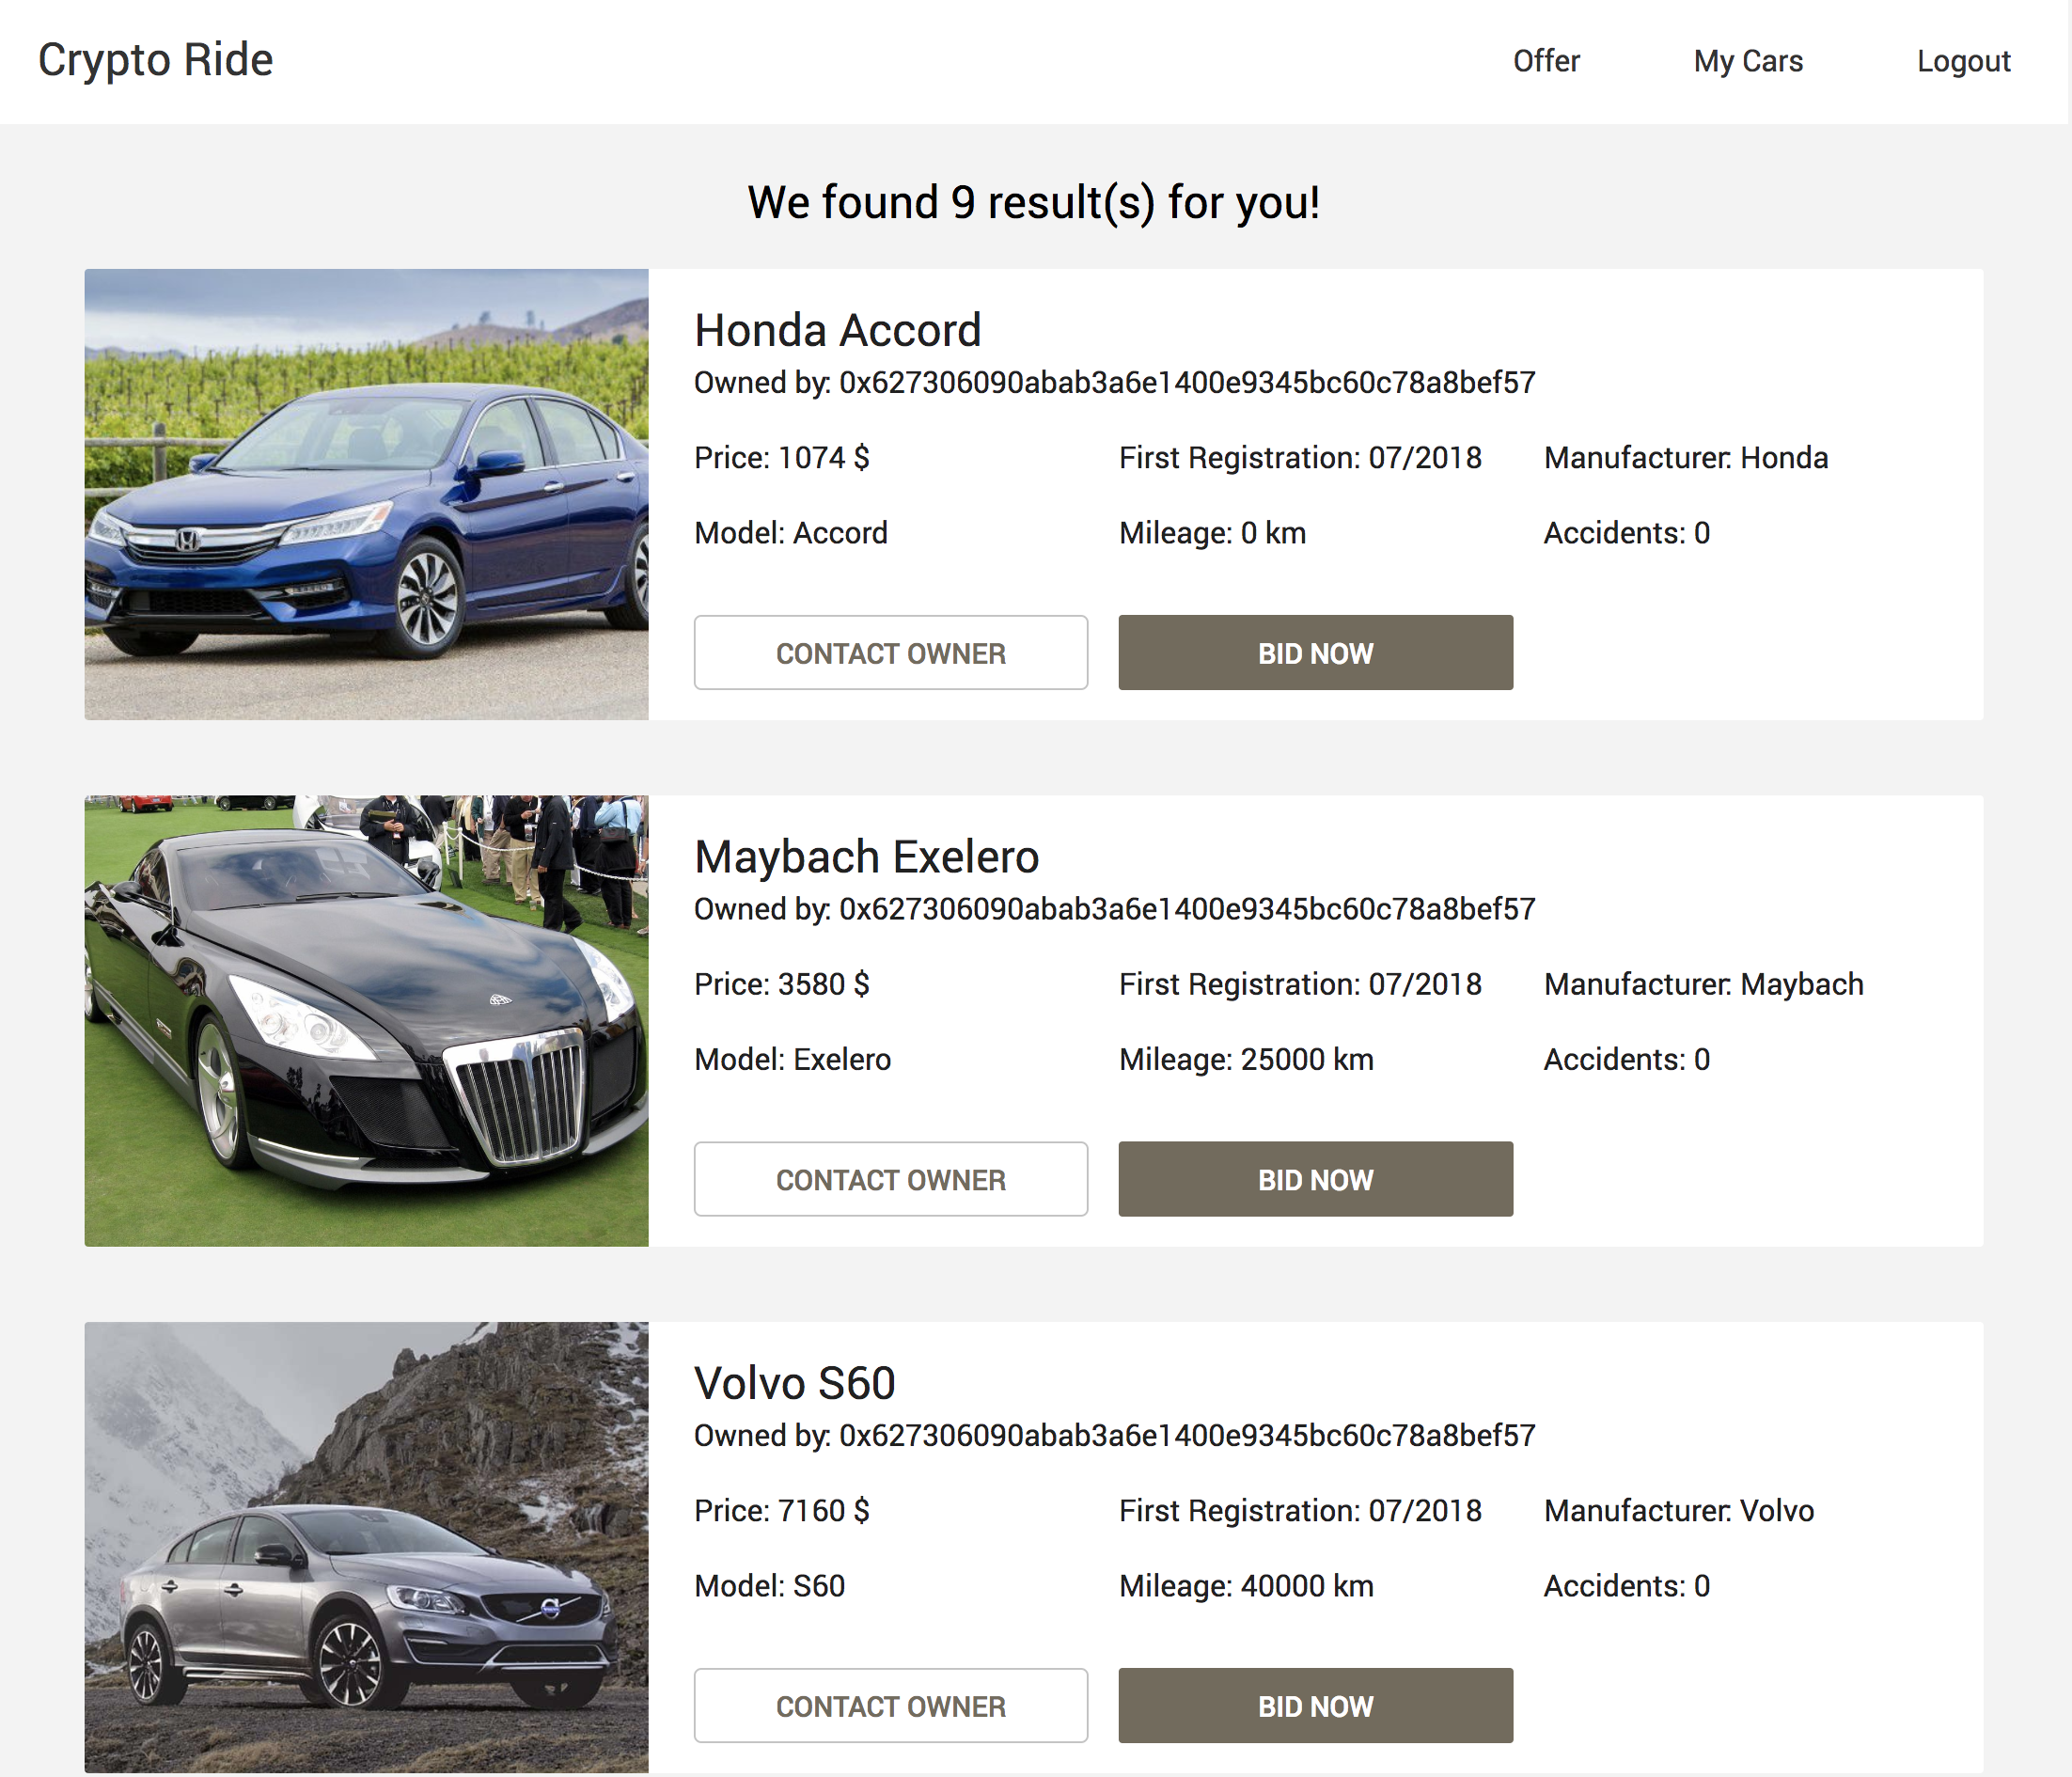
\includegraphics[width=1\textwidth]{figures/cryptoride_screens/offers_overview.png}}
% \caption{Screen: Overs overview \label{fig:screen_offers_overview}}
% \end{figure}

\clearpage
\section{Selling Points}\label{sec:selling_points}

Our implementation successfully utilizes blockchain technology for managing vital application data. Although this causes some non-trivial challenges, which need to be dealt with, it also provides many benefits to the users of our application. We will now take a look at some of the benefits of blockchains in the context of our application.
\begin{itemize}
  \item \textbf{Trust}: The decentralized nature of blockchains eliminates the necessity for third parties to validate transactions between interacting users. Users of our trading platform are able to interact with one another, sell and buy cars without the need of anyone to confirm or issue their transactions.
  \item \textbf{Transparency}: The Ethereum ledger is public and can be accessed by anyone. In our application we use the blockchain to manage information regarding car sales as well as sensitive car properties such as mileage. Due to the transparency of the blockchain, all users of our platform have access to this information and are able to make well-informed decisions on whether or not to buy a car.
  \item \textbf{Immutability}: Data stored in the blockchain cannot be altered retrospectively. This means that users can rest assured that vital information provided by the blockchain, such as mileage, has not been tempered with.
  \item \textbf{Availability}: Peer-to-peer blockchains consisting of numerous nodes do not have a single point of failure that may cause data loss or inability to operate. For this reason, the blockchain component of our application is fully operational at all times and is able to ensure that data provided or already present will continue to be available in the future.
  \item \textbf{Utilization}: A public blockchain may be used by many different applications. It is imaginable that the blockchain component of our application could also be used by other applications, such as other trading platforms. This may increase the number of platform providers from which customers can choose in the future, while retaining the same benefits.
  \item \textbf{Performance}: Although the transaction performance of blockchains is a critical topic, many promising efforts are already made to increase their performance significantly. This would potentially enable users of our application to issue transactions at a much higher pace than they could with traditional methods.
  \item \textbf{Lower Fees}: Unlike other trading platforms where you may have to pay a fee to use their services, our application only requires you to pay the price it costs to put your content onto the blockchain.
\end{itemize}
All in all, our application leverages many of the benefits that blockchains already provide and will further benefit from any future development in that area.

\clearpage
\section{Conclusion} \label{sec:conclusion}

In this work, we presented our implementation of a decentralized car marketplace that is built upon the Ethereum blockchain. With this, we intend to demonstrate how the architecture of a state-of-the art web application can be combined with the Ethereum blockchain, yielding a hybrid approach to a blockchain powered application. While we still rely on a centralized front-end, the important business logic is running decentralized in form of smart contracts on the Ethereum network. Further, we believe that this hybrid approach helps developers, as well as stakeholders and end users to build up confidence with blockchain technology in the context of smart mobility. To name one example: the use of Ethereum as our application's backbone is almost transparent to the end user and any interaction with the blockchain is designed as intuitive and simple as possible. At the same time our implementation manages to provide the desired benefits of blockchain technology.

While our implementation already provides a rich feature set that covers all the core functionality of a car marketplace platform, we identify some task that could be tackled in future work. First, we made some assumptions in Section~\ref{concept:assumptions}. It is still open to evaluate these assumptions from a business perspective. E.g, would car dealers be willing to join such an ecosystem, what are possible hindrances?
Secondly, in this paper we focused on the software development part and not on legal issues. Thus, the legal compliance needs to be assessed. Lastly, Ethereum is just one of many blockchain technologies and many new ones have since been proposed that claim to solve issues of existing ones~\cite{NeoWhitePaper, EOSWhitePaper}. Therefore, it might be of value to compare, in the context of this implementation, Ethereum with newly proposed platforms in order to assess whether they indeed manage to solve these issues.

\clearpage

% Generate the bibliography.
\bibliography{bibliography}
\bibliographystyle{unsrt}

\end{document}
